% Options for packages loaded elsewhere
\PassOptionsToPackage{unicode}{hyperref}
\PassOptionsToPackage{hyphens}{url}
\PassOptionsToPackage{dvipsnames,svgnames,x11names}{xcolor}
%
\documentclass[
  11pt,
]{article}
\usepackage{amsmath,amssymb}
\usepackage{iftex}
\ifPDFTeX
  \usepackage[T1]{fontenc}
  \usepackage[utf8]{inputenc}
  \usepackage{textcomp} % provide euro and other symbols
\else % if luatex or xetex
  \usepackage{unicode-math} % this also loads fontspec
  \defaultfontfeatures{Scale=MatchLowercase}
  \defaultfontfeatures[\rmfamily]{Ligatures=TeX,Scale=1}
\fi
\usepackage{lmodern}
\ifPDFTeX\else
  % xetex/luatex font selection
\fi
% Use upquote if available, for straight quotes in verbatim environments
\IfFileExists{upquote.sty}{\usepackage{upquote}}{}
\IfFileExists{microtype.sty}{% use microtype if available
  \usepackage[]{microtype}
  \UseMicrotypeSet[protrusion]{basicmath} % disable protrusion for tt fonts
}{}
\makeatletter
\@ifundefined{KOMAClassName}{% if non-KOMA class
  \IfFileExists{parskip.sty}{%
    \usepackage{parskip}
  }{% else
    \setlength{\parindent}{0pt}
    \setlength{\parskip}{6pt plus 2pt minus 1pt}}
}{% if KOMA class
  \KOMAoptions{parskip=half}}
\makeatother
\usepackage{xcolor}
\usepackage[margin=0.9in]{geometry}
\usepackage{longtable,booktabs,array}
\usepackage{calc} % for calculating minipage widths
% Correct order of tables after \paragraph or \subparagraph
\usepackage{etoolbox}
\makeatletter
\patchcmd\longtable{\par}{\if@noskipsec\mbox{}\fi\par}{}{}
\makeatother
% Allow footnotes in longtable head/foot
\IfFileExists{footnotehyper.sty}{\usepackage{footnotehyper}}{\usepackage{footnote}}
\makesavenoteenv{longtable}
\usepackage{graphicx}
\makeatletter
\def\maxwidth{\ifdim\Gin@nat@width>\linewidth\linewidth\else\Gin@nat@width\fi}
\def\maxheight{\ifdim\Gin@nat@height>\textheight\textheight\else\Gin@nat@height\fi}
\makeatother
% Scale images if necessary, so that they will not overflow the page
% margins by default, and it is still possible to overwrite the defaults
% using explicit options in \includegraphics[width, height, ...]{}
\setkeys{Gin}{width=\maxwidth,height=\maxheight,keepaspectratio}
% Set default figure placement to htbp
\makeatletter
\def\fps@figure{htbp}
\makeatother
\setlength{\emergencystretch}{3em} % prevent overfull lines
\providecommand{\tightlist}{%
  \setlength{\itemsep}{0pt}\setlength{\parskip}{0pt}}
\setcounter{secnumdepth}{-\maxdimen} % remove section numbering
% definitions for citeproc citations
\NewDocumentCommand\citeproctext{}{}
\NewDocumentCommand\citeproc{mm}{%
  \begingroup\def\citeproctext{#2}\cite{#1}\endgroup}
\makeatletter
 % allow citations to break across lines
 \let\@cite@ofmt\@firstofone
 % avoid brackets around text for \cite:
 \def\@biblabel#1{}
 \def\@cite#1#2{{#1\if@tempswa , #2\fi}}
\makeatother
\newlength{\cslhangindent}
\setlength{\cslhangindent}{1.5em}
\newlength{\csllabelwidth}
\setlength{\csllabelwidth}{3em}
\newenvironment{CSLReferences}[2] % #1 hanging-indent, #2 entry-spacing
 {\begin{list}{}{%
  \setlength{\itemindent}{0pt}
  \setlength{\leftmargin}{0pt}
  \setlength{\parsep}{0pt}
  % turn on hanging indent if param 1 is 1
  \ifodd #1
   \setlength{\leftmargin}{\cslhangindent}
   \setlength{\itemindent}{-1\cslhangindent}
  \fi
  % set entry spacing
  \setlength{\itemsep}{#2\baselineskip}}}
 {\end{list}}
\usepackage{calc}
\newcommand{\CSLBlock}[1]{\hfill\break\parbox[t]{\linewidth}{\strut\ignorespaces#1\strut}}
\newcommand{\CSLLeftMargin}[1]{\parbox[t]{\csllabelwidth}{\strut#1\strut}}
\newcommand{\CSLRightInline}[1]{\parbox[t]{\linewidth - \csllabelwidth}{\strut#1\strut}}
\newcommand{\CSLIndent}[1]{\hspace{\cslhangindent}#1}
\ifLuaTeX
\usepackage[bidi=basic]{babel}
\else
\usepackage[bidi=default]{babel}
\fi
\babelprovide[main,import]{american}
% get rid of language-specific shorthands (see #6817):
\let\LanguageShortHands\languageshorthands
\def\languageshorthands#1{}
\usepackage[dvipsnames]{xcolor}
\usepackage{microtype}
\usepackage{caption}
\usepackage{placeins}
\usepackage{float}
\floatplacement{figure}{H}
\captionsetup{font=small,labelfont=bf}
\setlength{\emergencystretch}{3em}
\raggedbottom
\AtBeginDocument{\hypersetup{pdfauthor={Human authorship TBD},pdfsubject={AI-assisted living research draft; human review TBD}}}
\ifLuaTeX
  \usepackage{selnolig}  % disable illegal ligatures
\fi
\usepackage{bookmark}
\IfFileExists{xurl.sty}{\usepackage{xurl}}{} % add URL line breaks if available
\urlstyle{same}
\hypersetup{
  pdftitle={From Lexical Similarity to Contextual Comparison},
  pdflang={en-US},
  colorlinks=true,
  linkcolor={MidnightBlue},
  filecolor={Maroon},
  citecolor={MidnightBlue},
  urlcolor={MidnightBlue},
  pdfcreator={LaTeX via pandoc}}

\title{From Lexical Similarity to Contextual Comparison}
\usepackage{etoolbox}
\makeatletter
\providecommand{\subtitle}[1]{% add subtitle to \maketitle
  \apptocmd{\@title}{\par {\large #1 \par}}{}{}
}
\makeatother
\subtitle{A provenance-aware study of the Ra published sessions and
Bashar-related recordings}
\author{}
\date{Living research draft · 7 November 2026 · Run04 and official
follow-on}

\begin{document}
\maketitle

\textbf{Research status.} This is an AI-assisted research draft, not a
peer-reviewed publication. Human authorship, expert annotation and human
methodological review are \textbf{TBD}. The study compares retained
documents and their production contexts. It does not authenticate
attributed communicators, test extraterrestrial origins, validate
medical claims, or estimate the truth of metaphysical propositions. No
venue compliance or scholarly priority is claimed.

\FloatBarrier

\section{Abstract}\label{abstract}

Public material associated with channeling combines edited dialogues,
interviews, promotional excerpts, commentary and written teaching
summaries. Treating these materials as interchangeable speech can turn
genre or transcription artifacts into apparent differences between
teachings. We present a reproducible exploratory comparison of 106
numbered Ra sessions in the \emph{Lightly Edited} edition and 19
retained Bashar-related publisher recordings, comprising 501,300
whitespace words. Five official Bashar written pages are kept as a
separate reference stratum; 35 partly extracted handouts are excluded
from complete-text models. The analysis combines declared word-form
dictionaries, controlled TF-IDF similarities, nonnegative matrix
factorization, clustering, a document network, a frozen neural embedding
baseline and a documentary question/response database. Name-filtered
mean TF-IDF cosines are 0.3508 within the Bashar-related recordings,
0.1460 within Ra and 0.0929 across contexts. With centered 1,500-token
windows, these become 0.1620, 0.1070 and 0.0558. A two-cluster solution
follows source context but has a low cosine silhouette of 0.0929.
Contextual inspection of the highest corrected neural question-retrieval
leads reveals broad thematic overlaps alongside misleading matches
caused by generic wording, different referents and mixed prompt/response
segments. A separately frozen follow-on admits 84 English official
publications as 82 exact-media units; its 75 ordinary excerpt units
retain greater similarity to the mixed Bashar contexts than to Ra under
both full-text and length-controlled representations, while their
internal clusters are weak and unstable. Bounded source reading
identifies unity-oriented and agency-related parallels while preserving
differences in practice, time framing, ethical terminology and
qualifications. The results support provenance-aware exploration and
source-linked comparison; they do not isolate doctrinal causes from
period, editing, genre, speaker mixture or recognition effects.

\FloatBarrier

\section{1. Introduction}\label{introduction}

A comparison of two attributed bodies of teaching first requires a
decision about what is being compared. A numbered published dialogue, a
contemporary interview about that dialogue, a host's summary, a critical
retelling and an official instructional page can all contain the same
name while representing different speech acts. The speaker, narrator,
publisher, quoted source and subject of discussion may be different.
Downloading a file establishes availability of a particular edition; it
does not establish that every sentence belongs to the person or entity
named in its title.

This problem is especially consequential when a project asks whether
Bashar-related material resembles the Ra material. The retained Ra
collection provides an organized sequence of edited sessions with
printed documentary roles. The initial Bashar-related recordings provide
much longer contemporary conversations with unidentified speakers,
interruptions and sometimes advertisements. Their dates, editorial
histories and recording conditions differ. A model can separate these
collections accurately while learning the differences between edited
dialogue and conversational media rather than a substantive contrast
between the teachings.

Our purpose is to make these distinctions inspectable. We combine
quantitative maps with a bounded reading layer that records both
apparent parallels and failed matches. The analysis asks where
vocabulary recurs, how sensitive its patterns are to preprocessing and
document length, and what a closer reading does to a proposed semantic
match. It treats computational processing, semantic inspection and
empirical verification as separate activities. Processing every word
with an encoder is not the same as reading every document for meaning;
reading a statement is not verification of its content.

The contribution of this draft is a traceable case study and
implementation, not a claim to have discovered a common origin or a
definitive taxonomy of channeling. It provides a typed source inventory,
multiple lexical controls, complete chunk coverage for a pinned neural
baseline, a private database that preserves documentary and uncertain
roles, and public paraphrases linked to specific questions or recording
intervals. The living-paper format is intended to accommodate new
acquisitions without silently changing the denominator of an earlier
result.

\FloatBarrier

\section{2. Background and related methodological
work}\label{background-and-related-methodological-work}

\FloatBarrier

\subsection{2.1. Source context as an analytical
variable}\label{source-context-as-an-analytical-variable}

Here, \emph{Ra} identifies the published sessions collected from
lawofone.info in its Lightly Edited edition. \emph{Bashar-related}
identifies retained publisher material whose titles or descriptions
associate it with Bashar or Darryl Anka. These are source-context
labels. They are not independently verified identities of every voice.
Five official written teaching pages provide a more direct
publisher-attributed reference layer, while official handouts and public
excerpts provide additional modalities and scopes.

This distinction follows the rationale of data statements: curation
decisions, language, speech situations, producers, annotators and
upstream resources affect what a language dataset can support
(\citeproc{ref-bender2018}{Bender and Friedman 2018}). The
data-statement approach motivates recording whether a passage is edited
prose or spontaneous speech, whether it is a host question or a printed
response, and whether recognition or optical character recognition has
intervened. It does not itself resolve the differences among these
strata.

\FloatBarrier

\subsection{2.2. Topic interpretation and numerical
stability}\label{topic-interpretation-and-numerical-stability}

Topic models produce mathematical decompositions that need
interpretation. Top words are useful browsing aids, but neither
coherence nor a low reconstruction error certifies that a component
corresponds to a meaningful or consistently used concept. Doogan and
Buntine argue for assessing representative documents alongside word
lists and show limits of aggregate interpretability measures in their
specialized-domain evaluation (\citeproc{ref-doogan2021}{Doogan and
Buntine 2021}). Our source-linked reading and explicit counterexamples
adopt that principle. Their human subject-matter-expert evaluation is
not reproduced here.

Reliability also differs from similarity between repeated fits.
Schroeder and Wood-Doughty distinguish reliability questions from common
topic-similarity diagnostics; their empirical work concerns LDA, with
other model families left for further study
(\citeproc{ref-schroeder2025}{Schroeder and Wood-Doughty 2025}). We
therefore report NMF component matching and KMeans seed agreement as
numerical diagnostics, not as validated reliability coefficients. In
particular, nearly identical structured initializations provide a narrow
perturbation, and additional components can reduce reconstruction error
without becoming more interpretable.

\FloatBarrier

\subsection{2.3. Speech recognition and
leakage}\label{speech-recognition-and-leakage}

The retained ASR is evidence about what a recognition system produced.
It has not been audited against a representative audio sample. The
author-posted abstract of Koenecke and colleagues reports invented
phrases or sentences in a Whisper evaluation and associations with
non-vocal durations (\citeproc{ref-koenecke2024}{Koenecke et al. 2024}).
Those results motivate retaining audio and checking uncertain claims;
the study's rates and speaker populations cannot be transferred to this
collection. Recognition errors may affect negation, names, numbers and
turn boundaries, all of which matter to comparative interpretation.

Kapoor and Narayanan's abstract-level account of leakage and
reproducibility problems motivates explicit source-family and evaluation
boundaries (\citeproc{ref-kapoor2023}{Kapoor and Narayanan 2023}).
Excerpts from the same recording, alternate editions and reposts should
not be split as if independent observations in a future predictive
evaluation. The present analysis is descriptive and does not report a
held-out classifier accuracy. It therefore does not claim to have solved
a supervised leakage problem or to demonstrate generalization to
independent creators.

Access depth matters to these citations. Three official ACL PDFs were
retrieved and selected pages inspected: Doogan and Buntine, PDF pages 1,
4, 6 and 9; Schroeder and Wood-Doughty, pages 1, 2 and 9; Bender and
Friedman, pages 1, 4 and 5. The Kapoor--Narayanan and Koenecke et
al.~works were bibliographically verified through Crossref, but only
their author-posted arXiv abstracts and version histories were read.
Full-paper claims about those two studies are outside this draft. The
companion \texttt{REFERENCES.md} records these limits and the retained
earlier bibliography; this is not a comprehensive systematic literature
review.

\FloatBarrier

\section{3. Research questions}\label{research-questions}

The analysis addresses four exploratory questions:

\begin{enumerate}
\def\labelenumi{\arabic{enumi}.}
\tightlist
\item
  \textbf{RQ1 --- Collection and structure:} What is retained, in which
  editions and formats, and how much of it enters each analysis?
\item
  \textbf{RQ2 --- Lexical organization:} Which word-form patterns, topic
  decompositions, clusters and document neighborhoods appear, and how do
  they change under document-length and source-format controls?
\item
  \textbf{RQ3 --- Retrieval and dialogue:} What does neural similarity
  retrieve across the collections, and does contextual inspection
  support a common question or an equivalent answer?
\item
  \textbf{RQ4 --- Substantive comparison:} Within explicitly inspected
  sources, what parallels and differences arise in ontology, agency,
  ethics, fear, practice, time, contact, healing, knowledge and
  relationships?
\end{enumerate}

No directional hypotheses were preregistered. No hypothesis tests,
p-values, confidence intervals for an independent creator population, or
probabilities of an extraterrestrial origin are estimated. Proposed
confirmatory studies appear later as \textbf{TBD}, rather than as
results of this exploratory work.

\FloatBarrier

\section{4. Data, provenance and units}\label{data-provenance-and-units}

\FloatBarrier

\subsection{4.1. Frozen primary corpus}\label{frozen-primary-corpus}

The primary fitted frame contains 125 documents: 106 numbered Ra
sessions and 19 Bashar-related publisher recordings. The Ra source dates
span 15 January 1981 to 15 March 1984. The retained recording
publication dates span March 2022 to March 2026; publication time does
not necessarily identify the original spoken event. These date types are
displayed separately. Five official written references add contextual
material but do not fit the primary lexical models.

\begin{longtable}[]{@{}
  >{\raggedright\arraybackslash}p{(\columnwidth - 6\tabcolsep) * \real{0.3100}}
  >{\raggedleft\arraybackslash}p{(\columnwidth - 6\tabcolsep) * \real{0.1000}}
  >{\raggedleft\arraybackslash}p{(\columnwidth - 6\tabcolsep) * \real{0.1400}}
  >{\raggedright\arraybackslash}p{(\columnwidth - 6\tabcolsep) * \real{0.4500}}@{}}
\toprule\noalign{}
\begin{minipage}[b]{\linewidth}\raggedright
Stratum
\end{minipage} & \begin{minipage}[b]{\linewidth}\raggedleft
Docs
\end{minipage} & \begin{minipage}[b]{\linewidth}\raggedleft
Whitespace words
\end{minipage} & \begin{minipage}[b]{\linewidth}\raggedright
Role in this draft
\end{minipage} \\
\midrule\noalign{}
\endhead
\bottomrule\noalign{}
\endlastfoot
Ra Lightly Edited published sessions & 106 & 278,601 & Primary fitted
corpus; printed roles retained \\
Bashar-related publisher ASR & 19 & 222,699 & Primary fitted corpus;
unknown/mixed speakers \\
Official Bashar written pages & 5 & 1,646 & Separate reference
projection and reading \\
Official session-handout PDFs & 35 & Not used as a complete-text
denominator & Excluded from fitting because text extraction is
partial \\
Official English publication texts & 84 & 69,166 & Separate final
follow-on; 82 exact-media model units, outside the primary fit \\
\end{longtable}

The final official follow-on assigns a disposition to each of 87
publications in its finite player census. It admits 84 English
publication texts, holds two acquired multilingual texts outside the
English analysis, and excludes one source whose measured duration is
299.648 seconds despite its rounded 300-second discovery label. Two
verified exact-media duplicate pairs reduce the 84 English publications
to 82 model units containing 67,536 words. Of these, 75 are ordinary
excerpts, four are promotional or product material, and three are
greetings. The initial 15-publication snapshot---14 platform
auto-caption tracks and one local ASR output, 12,589 words---remains
preserved as historical acquisition evidence. Only the 870-word
local-ASR pilot has been inspected semantically in full. Neither this
expanded acquisition nor its separate modeling changes the original
fitted denominator.

The 19 recordings comprise 17 interviews, one promotional interview and
one skeptical commentary. They are not 19 authenticated channeling
sessions. The Ra collection is complete with respect to the selected 106
published pages. The publisher notes that editing and prior printed
sources can reconstruct gaps in surviving audio. Thus text completeness
is not original-tape completeness. Similarly, a complete public excerpt
remains partial with respect to a longer paid session.

\begin{figure}
\centering
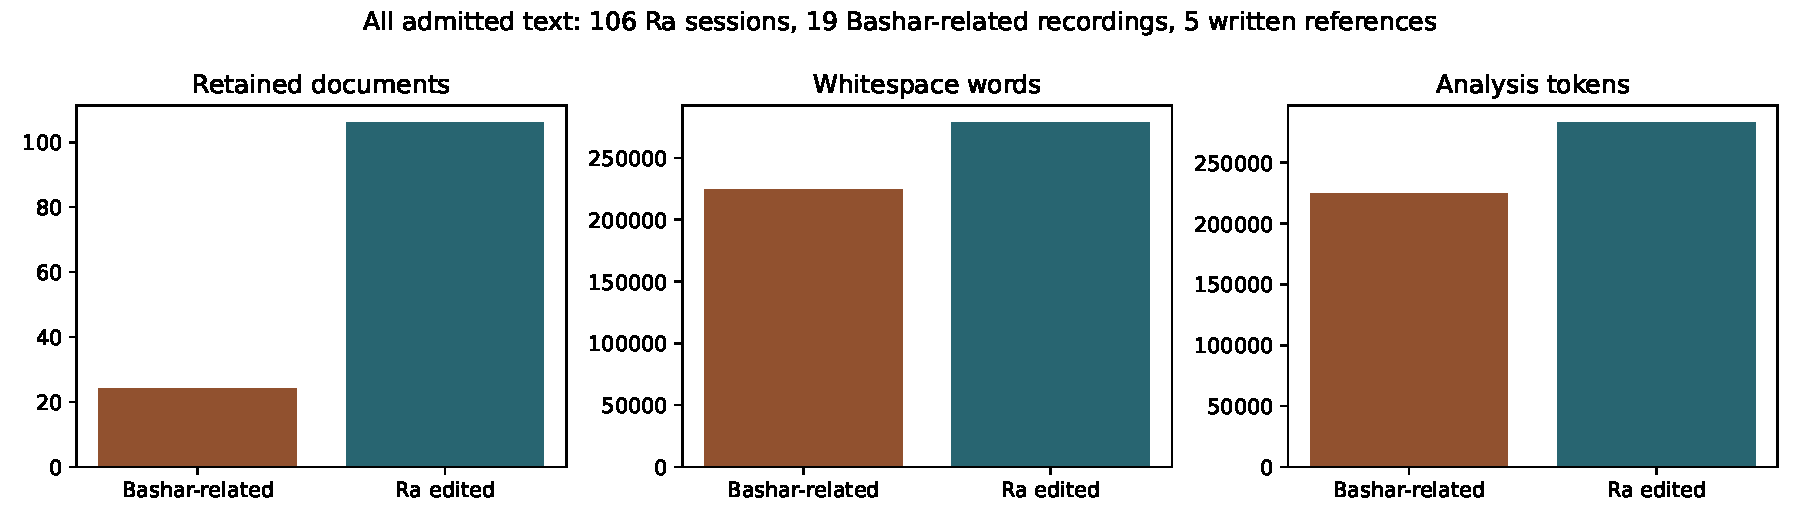
\includegraphics[width=0.95\textwidth,height=\textheight]{figures/corpus-coverage.pdf}
\caption{Admitted documents and words. The bars include five separate
official written references; only the 125 session/recording documents
fit primary lexical models. Counts are not independent creators or
authenticated speakers.}
\end{figure}

\FloatBarrier

\subsection{4.2. Evidence contracts and
exclusions}\label{evidence-contracts-and-exclusions}

Every admitted record binds normalized text and original evidence
through source IDs, paths, byte lengths and SHA-256 hashes. The
normalized text must equal the newline-joined ordered turn texts. Ra
extraction receipts are checked against the retained pages; ASR text,
segment order and timestamps are checked against completed original
receipts and media hashes. Missing or changed evidence for a completed
record stops analysis. These checks establish consistency of retained
bytes and provenance, not the accuracy of recognition or source claims.

Partial or failed text records are explicit exclusions. Thirty-five
handouts are excluded because text-only extraction omits visual
relationships or produces corrupted OCR. Three inspected page images
demonstrate why this matters: the Parallel Realities extraction retains
almost only the title, and the Nine Levels image contains a structured
table whose rotated OCR is damaged. Their visual meaning cannot be
recovered from a nominally nonempty text file.

Exact repeated source records and exact text aliases are counted once;
none were found in this snapshot. A five-token shingle screen checks
possible overlap without declaring every shared phrase a duplicate. No
pair passed the implemented screening thresholds among 7,750 primary
pairs. This does not rule out re-encoding, paraphrase, excerpts or
shared original sessions. The original-session identity of many
recordings remains unresolved.

\FloatBarrier

\subsection{4.3. Ethical and publication
boundary}\label{ethical-and-publication-boundary}

The public release contains metadata, code, numerical summaries, figures
and bounded paraphrases with source locators. Raw copyrighted text,
substantial excerpts, audio, source PDFs and the full private question
database are not republished with the paper. Public availability does
not establish an open training or redistribution license. Source
statements concerning health, suffering or abuse are analyzed as claims;
their inclusion does not endorse causation, assign blame or supply
clinical guidance.

\begin{figure}
\centering
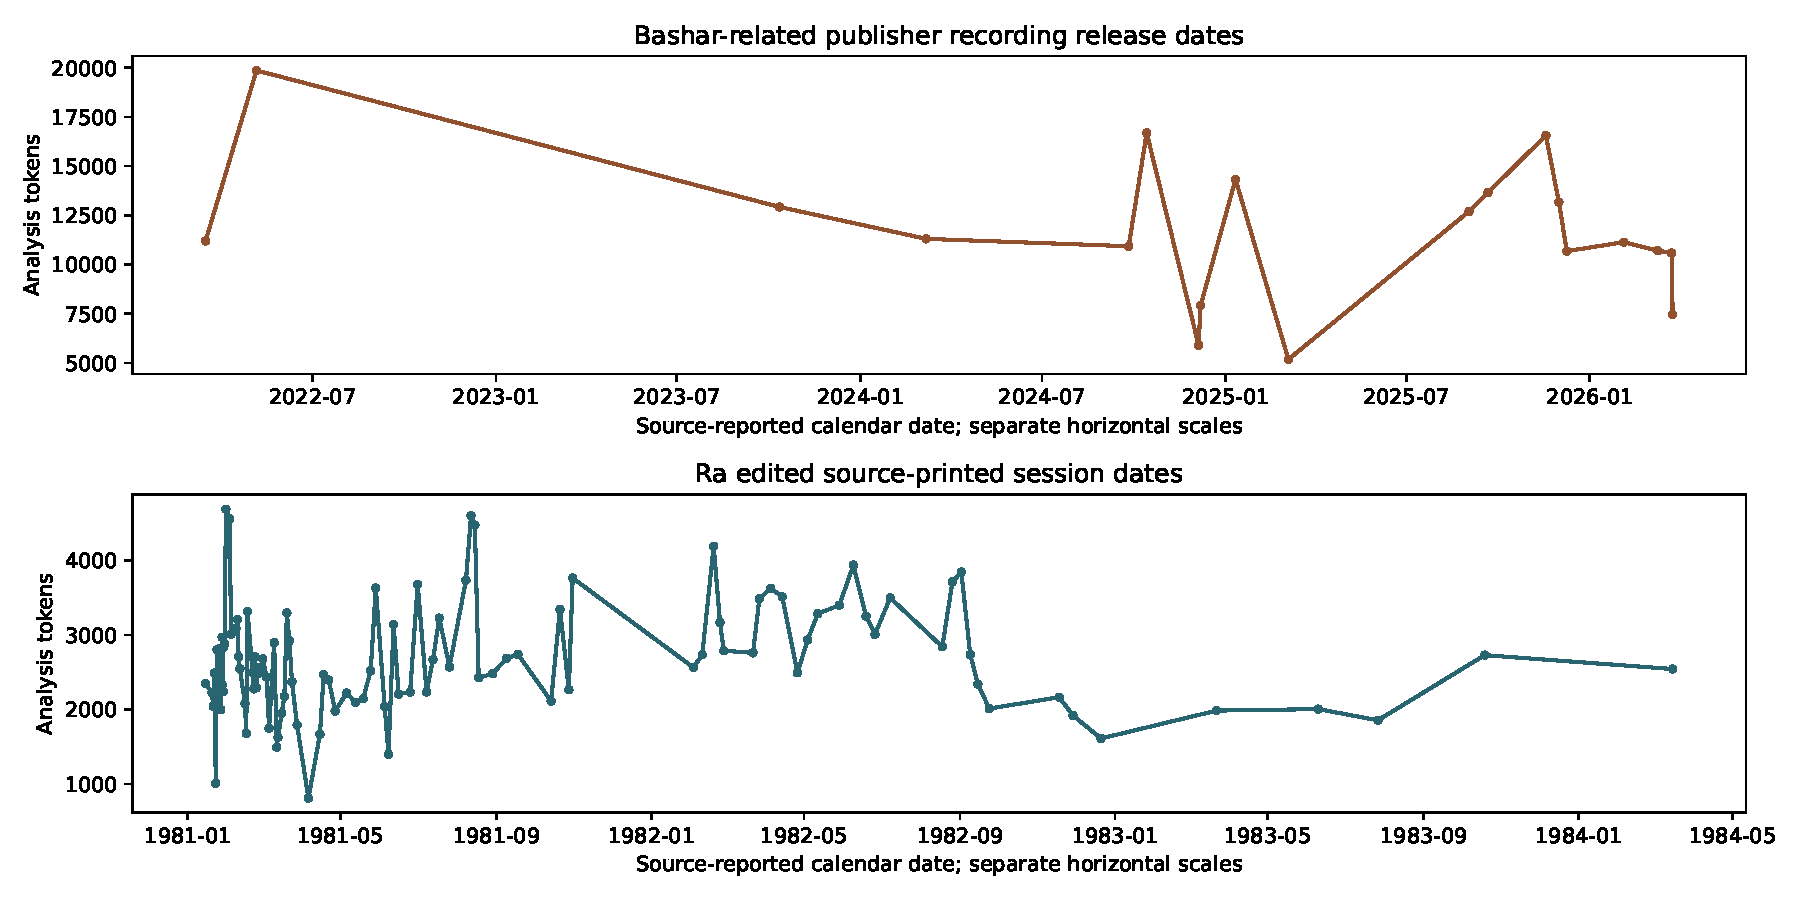
\includegraphics[width=0.95\textwidth,height=\textheight]{figures/chronology.pdf}
\caption{Primary chronology, on separate source-context scales. Ra
session dates and contemporary publication dates are different temporal
variables; undated written references are omitted. This is an inventory
view, not an aligned natural experiment.}
\end{figure}

\FloatBarrier

\section{5. Methods}\label{methods}

\FloatBarrier

\subsection{5.1. Tokenization and dictionary
comparison}\label{tokenization-and-dictionary-comparison}

The analysis normalizes Unicode with NFKC, standardizes curly
apostrophes, lowercases text and extracts ASCII-letter words with
internal apostrophes. These analysis tokens differ from whitespace
words. The primary collection contains 505,748 analysis tokens: 282,966
Ra and 222,782 Bashar-related tokens. English assumptions and the
stoplist are explicit; no multilingual validity is asserted.

Ten declared dictionaries operationalize word-form groups: ontology,
agency/free will, ethics/polarity, fear, practices, time/probability,
contact, healing/body, knowing/uncertainty and relationships. For
document \(d\) and group \(g\), the rate is \(r_{dg}=1000m_{dg}/n_d\),
where \(m_{dg}\) counts exact listed forms and \(n_d\) is the document's
analysis-token count. An equal-document mean gives each session or
recording equal weight; a pooled rate weights by text length. These
measures count words in questions, negations, quotations, advertisements
and skeptical restatements as well as affirmative claims. They are not
semantic classifications.

\FloatBarrier

\subsection{5.2. TF-IDF and
sensitivities}\label{tf-idf-and-sensitivities}

The joint vectorizer uses unigrams and bigrams, sublinear term
frequency, smoothed inverse document frequency, L2 row normalization, a
12,000-feature cap, \texttt{min\_df=2} for these sample sizes and
\texttt{max\_df=1.0}. English stop words retain \emph{no}, \emph{not},
\emph{nor} and \emph{never} at the stoplist stage. Preserving a negative
word does not make cosine an entailment model; feature selection and
pooling can still obscure its role. Similarity is the dot product of
normalized document vectors.

Seven variants make selected dependencies visible: raw vocabulary;
spoken fillers removed; fillers plus fixed names/source markers removed;
centered contiguous 1,500-token windows before filtering; Ra printed
responses only with Bashar ASR unchanged; bracketed spans removed; and
promotional/commentary source formats excluded. The response-only
variant is intentionally asymmetric because Bashar speaker roles remain
unidentified. The length control excludes four Ra sessions shorter than
1,500 tokens, leaving 121 documents. The format exclusion leaves 17
interviews and all 106 Ra sessions. Each variant refits its
vocabulary/IDF, so differences can reflect both retained text and
feature weights.

\FloatBarrier

\subsection{5.3. Topics, clusters and document
network}\label{topics-clusters-and-document-network}

NMF candidates use \(k=2\) through \(8\), seeds 11, 23 and 47, NNDSVDar
initialization, 800 maximum iterations and tolerance \(10^{-4}\).
Component vectors are matched across seeds using the Hungarian
algorithm. Reconstruction error, convergence warnings, iterations and
concentration diagnostics are retained. Four components are displayed
for readability; they are not a statistically selected optimal topic
count. Normalized component weights are decomposition shares, not
probabilities that a source holds a belief.

KMeans uses the name/source-marker-filtered vectors, ten
initializations, 500 maximum iterations, the same candidate counts and
seeds. The displayed solution maximizes the seed-11 cosine silhouette.
Corpus labels do not fit or select the solution. Adjusted-Rand agreement
assesses seed dependence, not doctrinal validity. A two-dimensional
TruncatedSVD projection supplies a visual arrangement; its axes are not
metaphysical dimensions.

The graph is the undirected union of each document's three nearest
lexical neighbors at cosine at least 0.15. Threshold counts from 0.10 to
0.50 are retained. Circular placement is schematic. Edges connect text
documents under this rule, not alleged beings or civilizations. Missing
cross-context edges can result from the nearest-neighbor rule and cannot
be interpreted as proof of unrelated ideas.

\FloatBarrier

\subsection{5.4. Frozen neural sensitivity and documentary
exchanges}\label{frozen-neural-sensitivity-and-documentary-exchanges}

The neural baseline is \texttt{all-MiniLM-L6-v2} from Sentence
Transformers, with separate hashes for the model, tokenizer and
configuration, and the complete pinned revision recorded in
\texttt{snapshot.json}. It is an established English baseline, not a
claim of state-of-the-art accuracy for this domain. No weights are
trained or edited. ONNX inference uses two intra-operation CPU threads,
one inter-operation thread and batches of 16.

Tokenization does not truncate content. Every document is split into
nonoverlapping chunks of at most 240 content wordpieces. Attention-mask
mean pooling includes the special tokens under the pinned pooling
contract; normalized chunk vectors are combined using content-token
counts and normalized again. Equal-chunk pooling is a sensitivity using
the same inference. Complete processed-wordpiece and chunk counts are
reported from the corrected frozen run below, with content truncation
explicitly checked. It still loses ordering across chunks and does not
interpret every proposition. Caches store float32 vectors, and replay
precision is checked separately; replay is not independent model
training.

Printed Ra questioner turns are paired with subsequent same-question-ID
response turns. Acknowledgments and requests to continue remain
documentary prompts. Lost-question notices, opening or orphan responses
and bracket-only turns remain explicit. Bashar ASR segments containing a
question mark produce punctuation candidates; the following segment is
context, not an automatically identified answer. The private SQLite
schema separates documents, turns, printed exchanges and ASR candidates.

Neural retrieval requires available question text, a question mark and
at least eight analysis tokens. It compares 2,311 Ra prompts with 775
Bashar ASR candidates. All eligible prompts, paired Ra responses and
candidates are fully encoded; the question layer records processed
wordpieces and checks for truncation. Ra prompt/response cosine is
summarized per session and contrasted with one cyclic reassignment of
responses within that session. A single shift is a descriptive
reference, not a null distribution or significance test.

\FloatBarrier

\subsection{5.5. Bounded qualitative
inspection}\label{bounded-qualitative-inspection}

The initial sample combines midpoint windows, a spread of 12 Ra sessions
and dictionary-enriched candidates. Its 50 unique windows contain 10,079
words: 22 Ra exchanges and 28 ASR windows. All were inspected by the
model. Nine further Ra exchanges supply conceptual depth and surrounding
context. All main text of five official written pages and three complete
handout page images were inspected separately. A later purposive audit
reads five initial high-cosine retrieval leads, their ASR neighborhoods
and three further Ra context exchanges. A corrected-run audit reuses the
first four exact pairs and inspects the changed fifth plus
Ra80.15--80.17, preserving the original fifth as a historical extra.

Cumulative inspection of the original collections covers 6,775 Ra words
across 32 sessions and 6,829 ASR words across all 19 recordings:
approximately 2.43\% and 3.07\% of their normalized words.
Complete-session semantic reading is not claimed. One new official
public excerpt contributes a separate full inspection of 870 ASR words
in 50 segments; the other supplementary excerpts are not thereby read or
validated. There is no human annotation, inter-rater agreement or
audio-listening validation. Sampling, offsets, hashes, counterexamples
and the distinction between original and follow-up coverage are
preserved in separate private attestations.

\FloatBarrier

\subsection{5.6. Separate official-publication
follow-on}\label{separate-official-publication-follow-on}

The follow-on preserves publication, edition and model-unit identities
separately. One text edition is selected per publication, preferring
available platform captions under a declared policy; that preference is
not an accuracy ranking. Original WebVTT cues are independently parsed
and compared with normalized text, order and timing. Local ASR is
checked against completed processing receipts, unchanged segment streams
and media hashes. Verified identical encoded-media hashes define one
model unit, while each publication remains in the source table and
question database. Metadata labels separate excerpts, greetings and
promotional/product material. They do not identify every speaker or
resolve all shared historical sessions.

Media admission checks packet continuity, with an additional
decoded-duration check for local-ASR editions. The retained admitted
media have no packet gaps above the declared 0.05-second tolerance.
Local-ASR editions must have container/decoded duration disagreement of
at most two seconds; platform-caption editions instead have audited
linked media and player/acquisition duration checks, without a
separately validated decoded-PCM duration. These checks caught an
earlier edition of \href{https://vimeo.com/204089777}{publication
204089777} with a 5.994667-second gap and a matching HTTP503
fragment-skip log. That edition and its receipts remain preserved but
rejected; a separately acquired strict replacement was recognized and
audited before fitting. Passing technical checks is not evidence that
the publisher excerpt contains a complete historical session or that
recognition is accurate.

The baseline vocabulary, IDF and NMF components remain fitted
exclusively to the original 125 documents and are numerically checked
against the accepted baseline before projection. A separate NMF
exploration fits the 75 ordinary official excerpt units; greetings and
promotional/product units do not enter that topic model. Four components
are displayed for readability, with candidate and seed diagnostics
retained. Centered 400-analysis-token controls use the frozen lexical
representation. Neural controls retain the corresponding contiguous
source span, including interior punctuation, numbers and case, after
declared Unicode and apostrophe normalization. Shorter documents are
excluded only from that sensitivity. This controls selected text length,
without matching historical period, speakers, editing or source
selection.

The original 19-context ASR used the bound tiny English Whisper model
with beam size one; new English excerpt ASR uses beam size five.
Platform caption settings are unknown. Explicitly translated
publications remain multilingual even when a recognizer returns a
dominant-language estimate. For two selected caption/local-ASR pairs,
token edit distance uses lowercased lexical tokens without punctuation
or stopword removal. Because both editions are machine outputs, the
measure is edition disagreement, not recognition accuracy or word error
rate against verified speech. Cue-interval coverage likewise measures
retained timestamp intervals rather than speech recall.

\FloatBarrier

\section{6. Results}\label{results}

\FloatBarrier

\subsection{6.1. Word forms describe different textual
emphases}\label{word-forms-describe-different-textual-emphases}

Table 2 gives equal-document dictionary rates per 1,000 analysis tokens.
Ra has higher rates in the declared ontology, ethics/polarity,
healing/body and practices groups. The retained interviews have higher
rates in the fear, contact and knowing/uncertainty groups. These are
observations about the listed words, not estimates of how much either
source genuinely discusses a validated psychological or doctrinal
construct. For example, \emph{know} can be conversational filler,
\emph{body} can be part of recurring Ra terminology, and \emph{positive}
or \emph{negative} can denote more than moral orientation.

\begin{longtable}[]{@{}
  >{\raggedright\arraybackslash}p{(\columnwidth - 4\tabcolsep) * \real{0.5000}}
  >{\raggedleft\arraybackslash}p{(\columnwidth - 4\tabcolsep) * \real{0.2500}}
  >{\raggedleft\arraybackslash}p{(\columnwidth - 4\tabcolsep) * \real{0.2500}}@{}}
\toprule\noalign{}
\begin{minipage}[b]{\linewidth}\raggedright
Declared word-form group
\end{minipage} & \begin{minipage}[b]{\linewidth}\raggedleft
Ra mean / 1,000
\end{minipage} & \begin{minipage}[b]{\linewidth}\raggedleft
Bashar-related mean / 1,000
\end{minipage} \\
\midrule\noalign{}
\endhead
\bottomrule\noalign{}
\endlastfoot
Ontology & 9.460 & 4.661 \\
Agency/free will & 6.362 & 5.228 \\
Ethics/polarity & 8.911 & 3.396 \\
Fear & 0.147 & 1.326 \\
Practices & 1.105 & 0.354 \\
Time/probability & 6.857 & 4.660 \\
Contact & 1.683 & 3.319 \\
Healing/body & 12.110 & 3.575 \\
Knowing/uncertainty & 3.763 & 10.146 \\
Relationships & 2.843 & 1.729 \\
\end{longtable}

The pooled-token rates generally preserve these directions but change
their magnitudes. For instance, ontology is 9.729 per 1,000 pooled Ra
tokens and 4.367 per 1,000 pooled recording tokens, compared with
equal-document means of 9.460 and 4.661. Equal-document weighting
prevents a long interview from dominating the context mean; it does not
make the 19 recordings representative of the larger available media
universe.

\begin{figure}
\centering
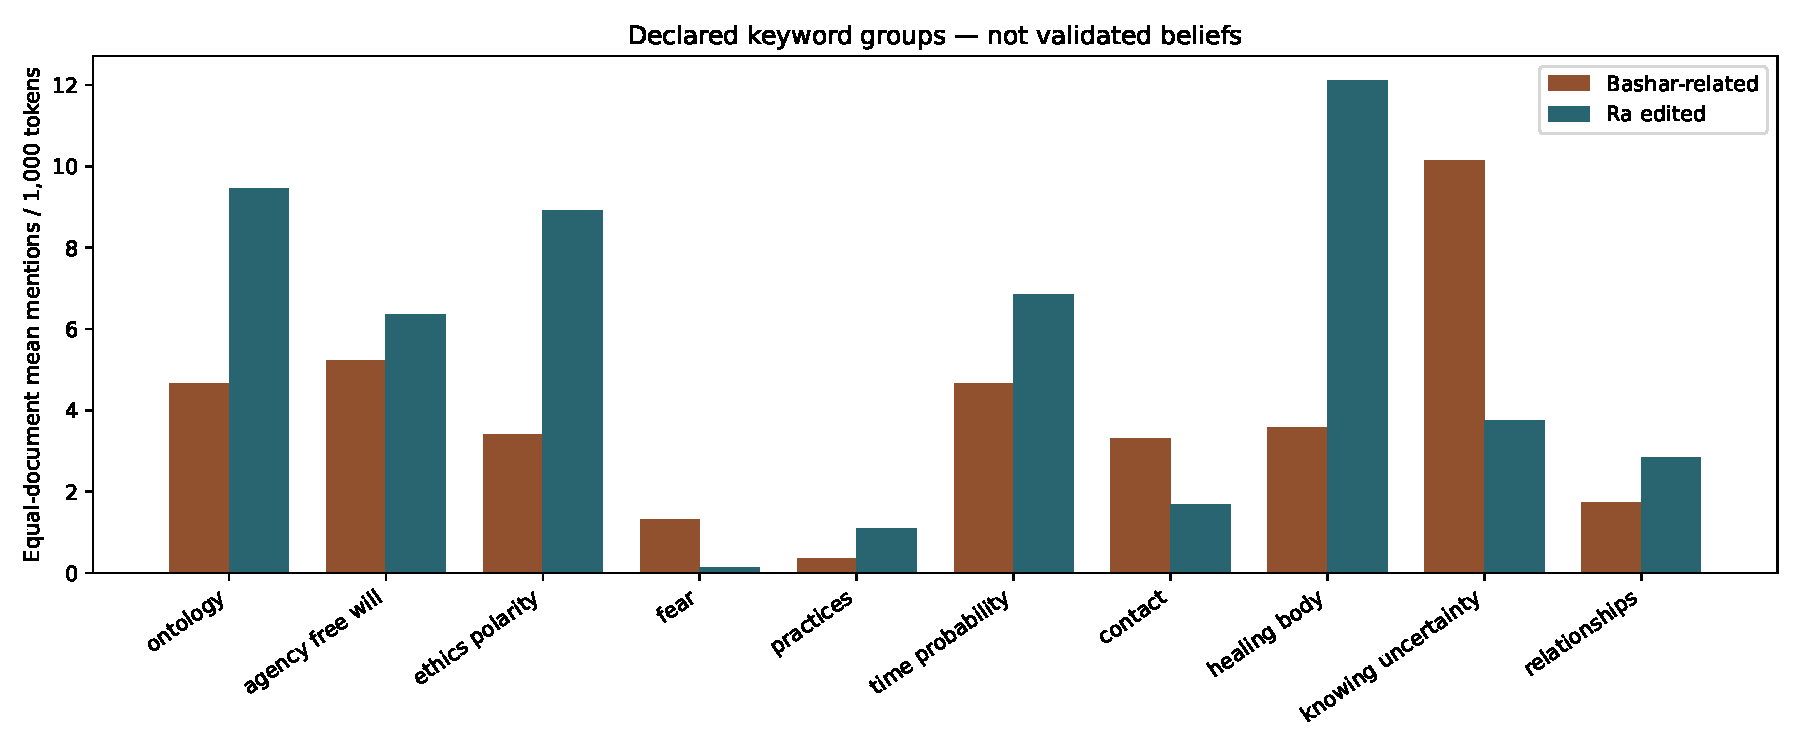
\includegraphics[width=0.95\textwidth,height=\textheight]{figures/keyword-comparison.pdf}
\caption{Declared word-form rates with equal document weights.
Pooled-token sensitivities and full dictionaries accompany the
machine-readable results. The groups are retrieval devices, not
validated semantic labels.}
\end{figure}

\FloatBarrier

\subsection{6.2. Lexical similarity is sensitive to document
length}\label{lexical-similarity-is-sensitive-to-document-length}

Within-context mean similarity exceeds across-context similarity in each
inspected lexical variant. The raw Bashar-related mean of 0.3862 falls
to 0.3508 when fixed spoken fillers and names/source markers are
removed. The Ra within mean falls from 0.1564 to 0.1460. Removing names
therefore does not eliminate source-context structure. It also does not
remove every host, genre, advertisement or editorial cue.

\begin{longtable}[]{@{}
  >{\raggedright\arraybackslash}p{(\columnwidth - 8\tabcolsep) * \real{0.4000}}
  >{\raggedleft\arraybackslash}p{(\columnwidth - 8\tabcolsep) * \real{0.1000}}
  >{\raggedleft\arraybackslash}p{(\columnwidth - 8\tabcolsep) * \real{0.1800}}
  >{\raggedleft\arraybackslash}p{(\columnwidth - 8\tabcolsep) * \real{0.1400}}
  >{\raggedleft\arraybackslash}p{(\columnwidth - 8\tabcolsep) * \real{0.1800}}@{}}
\toprule\noalign{}
\begin{minipage}[b]{\linewidth}\raggedright
TF-IDF variant
\end{minipage} & \begin{minipage}[b]{\linewidth}\raggedleft
Docs
\end{minipage} & \begin{minipage}[b]{\linewidth}\raggedleft
Bashar-related within
\end{minipage} & \begin{minipage}[b]{\linewidth}\raggedleft
Ra within
\end{minipage} & \begin{minipage}[b]{\linewidth}\raggedleft
Across contexts
\end{minipage} \\
\midrule\noalign{}
\endhead
\bottomrule\noalign{}
\endlastfoot
Raw & 125 & 0.3862 & 0.1564 & 0.0913 \\
Spoken fillers removed & 125 & 0.3554 & 0.1502 & 0.0915 \\
Fillers and fixed names removed & 125 & 0.3508 & 0.1460 & 0.0929 \\
Centered 1,500-token windows & 121 & 0.1620 & 0.1070 & 0.0558 \\
Ra responses only; ASR unchanged & 125 & 0.3605 & 0.1385 & 0.0798 \\
Bracketed spans removed & 125 & 0.3509 & 0.1460 & 0.0928 \\
Promotion and commentary excluded & 123 & 0.3628 & 0.1440 & 0.0924 \\
\end{longtable}

The length sensitivity is substantial. The within-recording mean changes
from 0.3508 to 0.1620, while the Ra within mean changes from 0.1460 to
0.1070. A whole long interview can share more broad vocabulary with
another long interview simply because both cover more subjects. The
centered-window comparison changes which content is observed and
excludes four short Ra sessions, so it is a sensitivity rather than an
identified estimate of a pure length effect. It nevertheless limits any
interpretation of the full-document contrast as a direct measure of
doctrinal consistency.

The complete primary comparison comprises 171 Bashar-related
within-context pairs, 5,565 Ra within-context pairs and 2,014
cross-context pairs. These overlapping pairs are not independent
observations: the same document contributes to many of them. We
therefore report descriptive means without treating thousands of
pairwise similarities as thousands of independent sources. The
response-only sensitivity also reduces the across-context mean, but it
cannot isolate a speaker effect because unidentified Bashar ASR remains
unchanged.

\begin{figure}
\centering
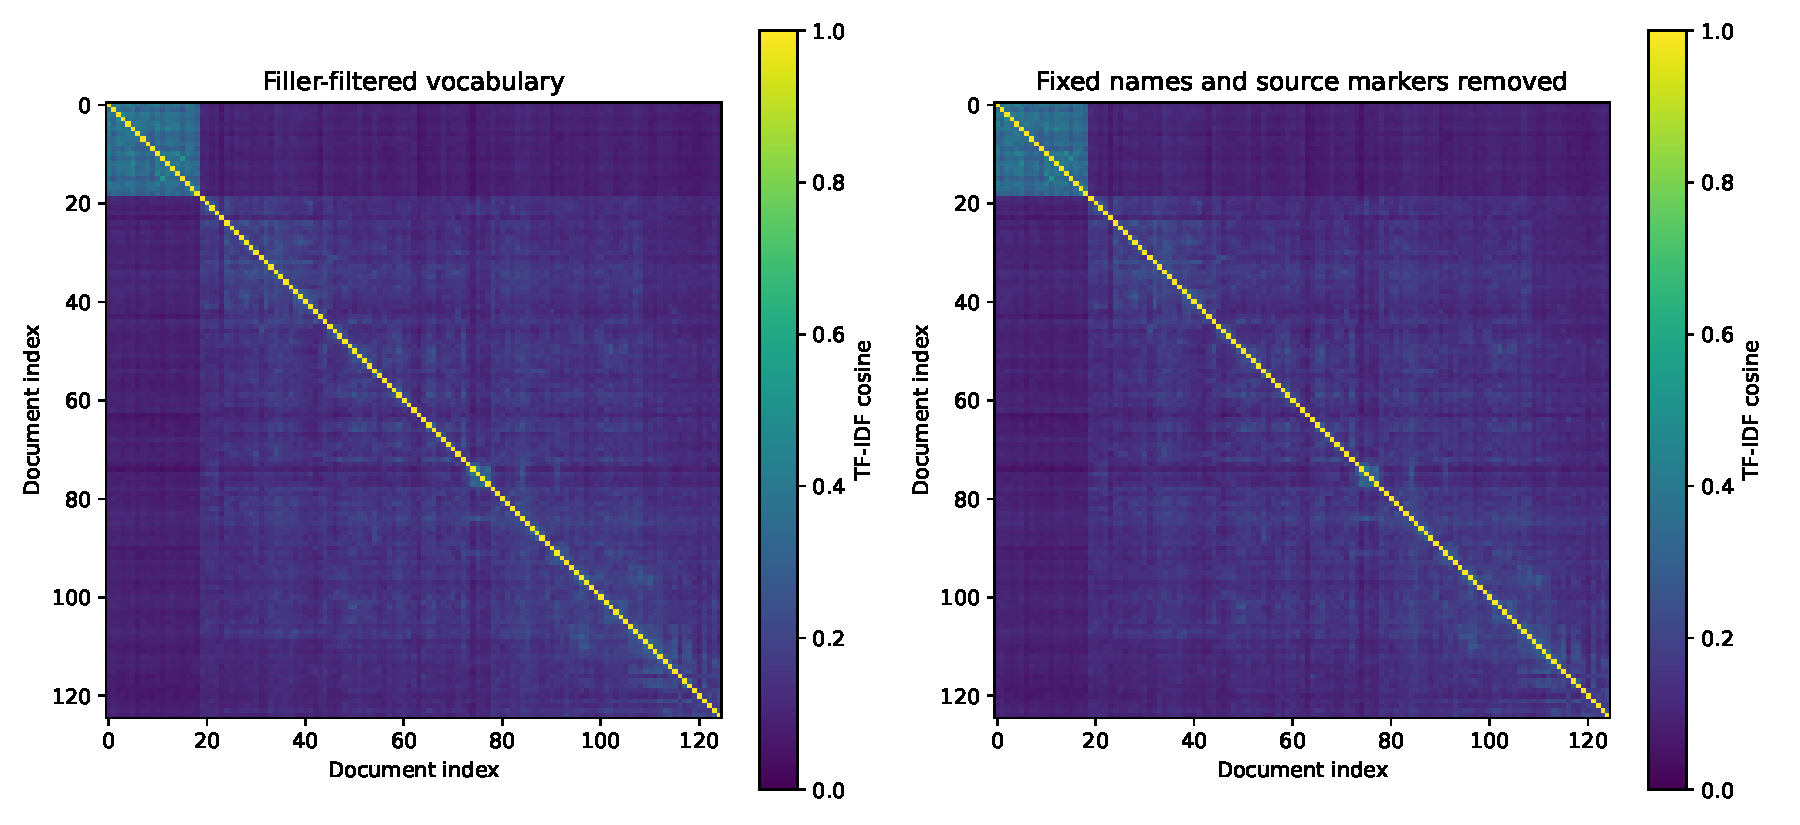
\includegraphics[width=0.85\textwidth,height=\textheight]{figures/lexical-similarity.pdf}
\caption{Name/source-marker-filtered lexical cosine matrix. Exact
document order and source IDs are in the data. Blocks indicate
vocabulary similarity under this representation, not agreement,
authenticity or a common origin.}
\end{figure}

\FloatBarrier

\subsection{6.3. Topic components expose source form as well as subject
matter}\label{topic-components-expose-source-form-as-well-as-subject-matter}

The four displayed NMF components have distinctive top-word patterns.
Component 1 includes density, entities, complex and Confederation
terminology. Component 2 combines reality, soul, frequency and passion
with remaining spoken forms. Component 3 emphasizes catalyst, mind, veil
and archetypical vocabulary. Component 4 emphasizes pyramid and chamber
terminology. Those labels summarize visible words; they are not
independent annotations of a latent doctrine.

\begin{longtable}[]{@{}
  >{\raggedright\arraybackslash}p{(\columnwidth - 6\tabcolsep) * \real{0.1600}}
  >{\raggedright\arraybackslash}p{(\columnwidth - 6\tabcolsep) * \real{0.4400}}
  >{\raggedleft\arraybackslash}p{(\columnwidth - 6\tabcolsep) * \real{0.2000}}
  >{\raggedleft\arraybackslash}p{(\columnwidth - 6\tabcolsep) * \real{0.2000}}@{}}
\toprule\noalign{}
\begin{minipage}[b]{\linewidth}\raggedright
Display component
\end{minipage} & \begin{minipage}[b]{\linewidth}\raggedright
Illustrative top terms
\end{minipage} & \begin{minipage}[b]{\linewidth}\raggedleft
Ra mean share
\end{minipage} & \begin{minipage}[b]{\linewidth}\raggedleft
Bashar-related mean share
\end{minipage} \\
\midrule\noalign{}
\endhead
\bottomrule\noalign{}
\endlastfoot
1 & density; entities; complex; confederation & 0.439 & 0.012 \\
2 & reality; lot; soul; physical reality; passion & 0.021 & 0.975 \\
3 & catalyst; mind; veil; archetypical & 0.399 & 0.007 \\
4 & pyramid; chamber; apex; spiraling & 0.141 & 0.006 \\
\end{longtable}

The concentration of the recordings in component 2 is an important
warning. It combines subject matter with conversational language, so it
may function partly as a broad source-format component. More components
are not automatically better: the six-component candidate reaches the
800-iteration limit for every seed. High agreement for several other
candidates occurs under NNDSVDar's closely related starting points and
should not be presented as stability under broad resampling, source
replacement or human interpretive review.

\begin{figure}
\centering
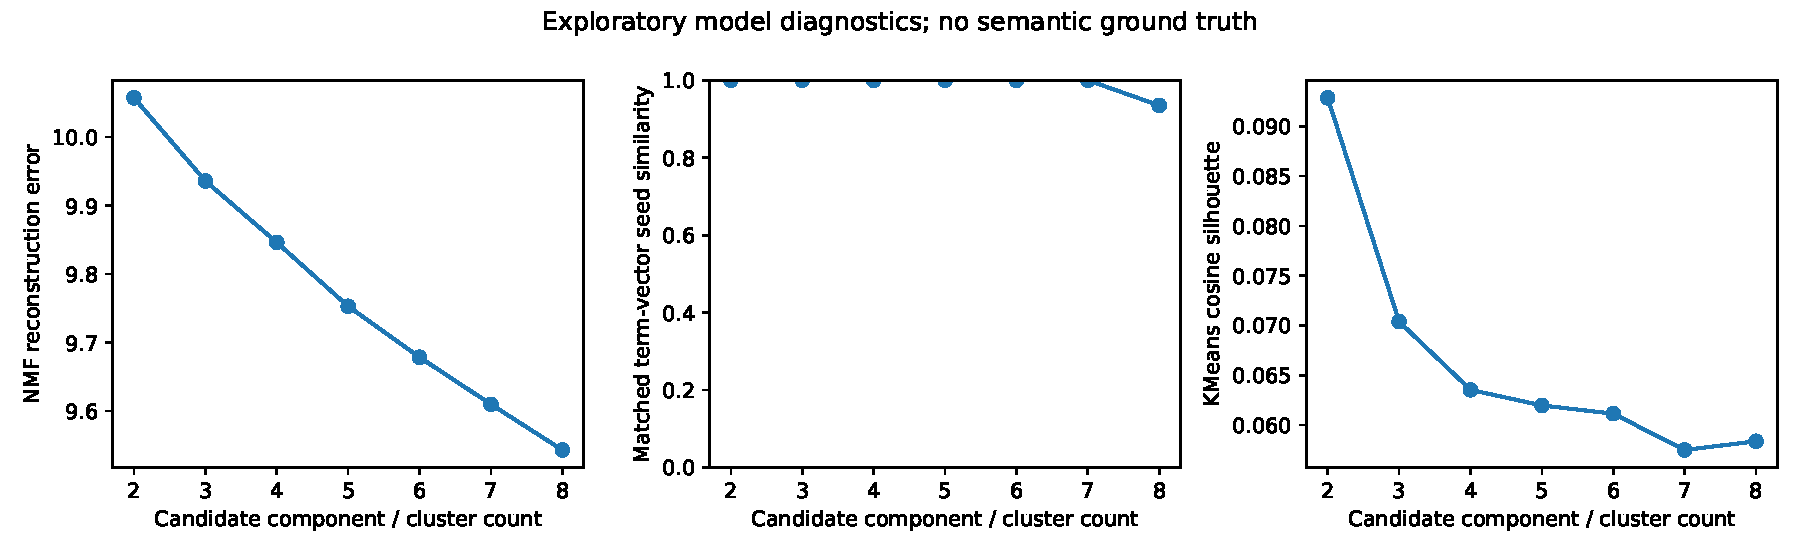
\includegraphics[width=0.95\textwidth,height=\textheight]{figures/topic-diagnostics.pdf}
\caption{Topic-model diagnostics across candidate counts. Reconstruction
error decreases as model capacity increases; seed matching and
convergence address different questions. The six-component candidate's
iteration-limit warning is retained.}
\end{figure}

\begin{figure}
\centering
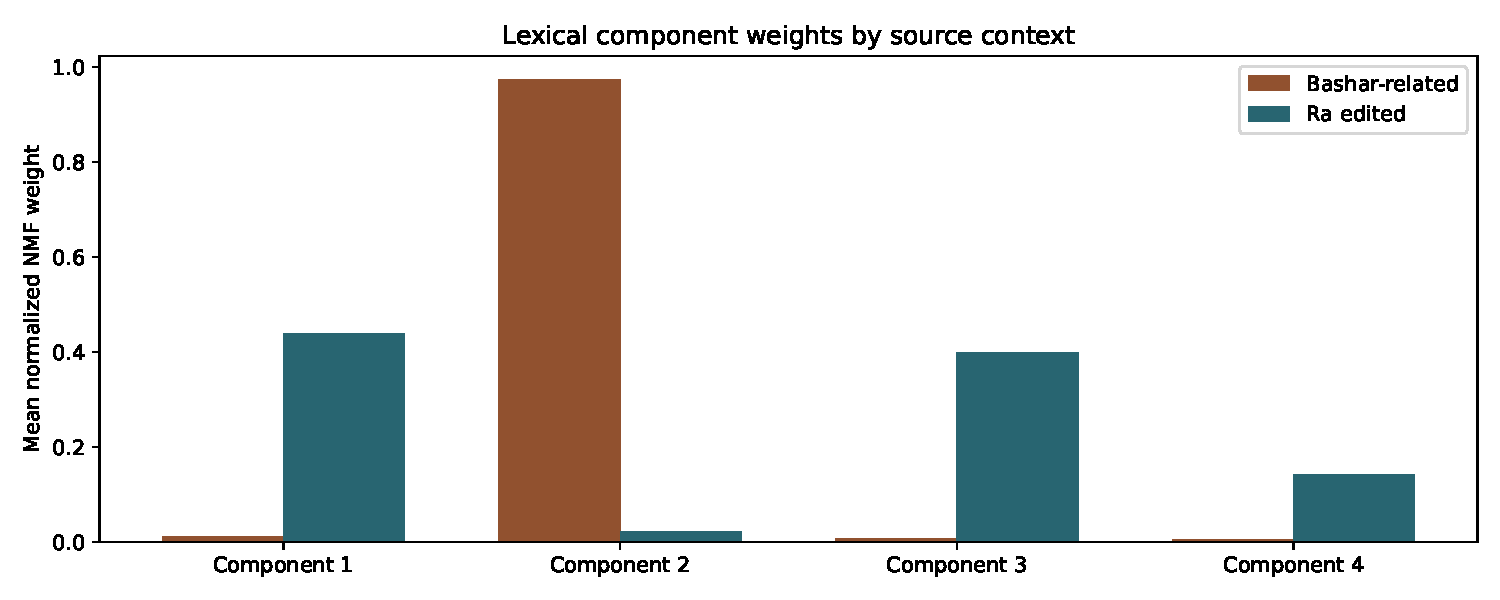
\includegraphics[width=0.9\textwidth,height=\textheight]{figures/topic-weights.pdf}
\caption{Mean normalized shares of the four displayed NMF components.
Shares are decomposition weights, not probabilities or a validated
estimate of how much a teaching endorses a topic.}
\end{figure}

\FloatBarrier

\subsection{6.4. Clusters and network neighborhoods follow source
context}\label{clusters-and-network-neighborhoods-follow-source-context}

The selected KMeans solution has two clusters of sizes 106 and 19,
aligning with the two source contexts, and a cosine silhouette of
0.0929. Seed adjusted-Rand agreement is 1.0 for this two-cluster
solution, while larger candidate partitions show lower agreement.
Reproducible assignment does not make the clusters substantive entities:
a low-separation partition can reliably distinguish edited sessions from
contemporary ASR while conflating period, editorial practice, host
speech and vocabulary.

The two-dimensional SVD display accounts for approximately 5.54\% of
variance through its reported two components. It is useful for
orientation but is a severe projection of a high-dimensional
representation. Visual distances in this map should not replace the
actual cosine matrix or imply a complete geometry of the documents.

\begin{figure}
\centering
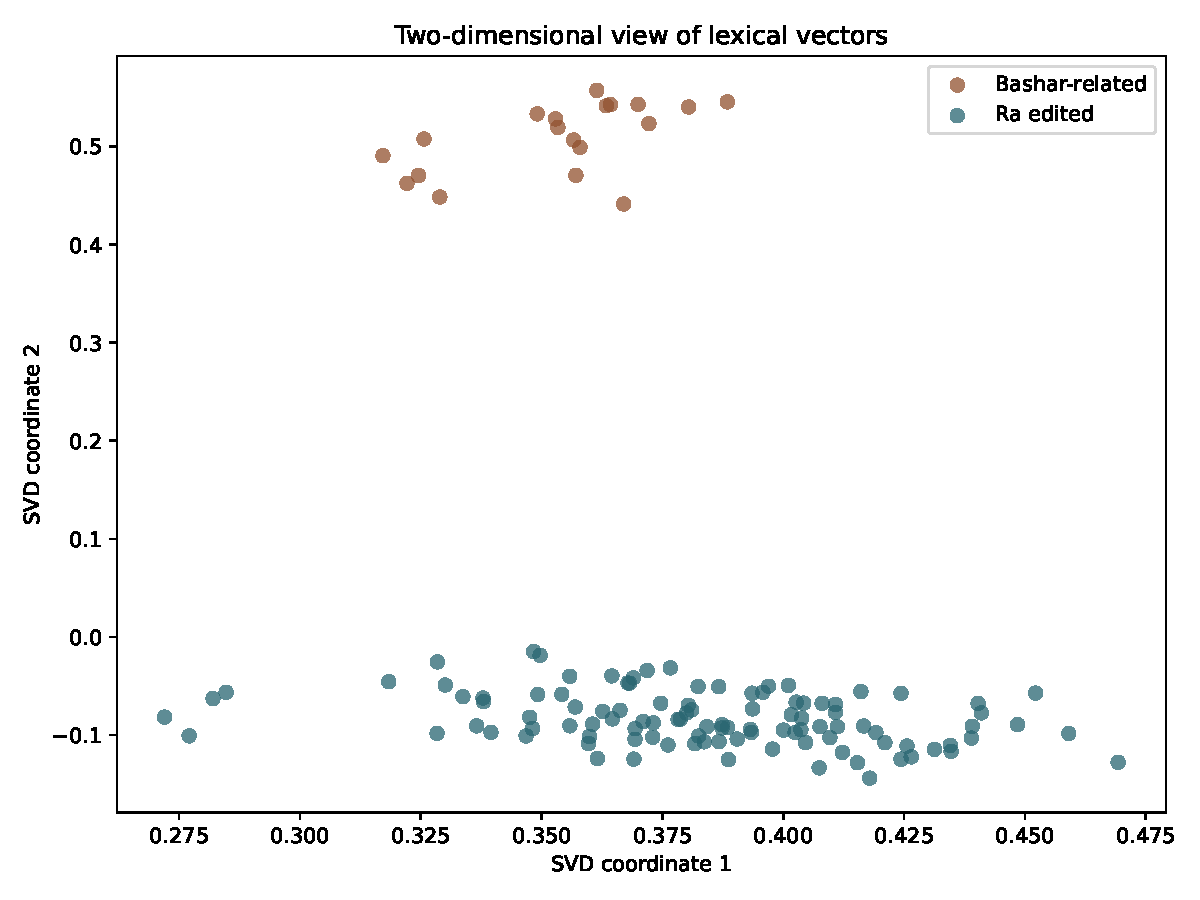
\includegraphics[width=0.9\textwidth,height=\textheight]{figures/cluster-map.pdf}
\caption{Two-dimensional lexical projection colored by source context.
Clustering uses the full representation; the display captures only a
small share of variance and its axes have no metaphysical
interpretation.}
\end{figure}

The three-nearest-neighbor graph at threshold 0.15 has 125 nodes and 266
edges, with no cross-context edges. Raising the threshold to 0.25 leaves
105 edges; at 0.50 only one remains. Even at 0.10 there are no
cross-context edges under this nearest-neighbor construction. This does
not imply zero cross-context similarity: the full matrix has a positive
across-context mean. It means that no cross-context document enters the
retained top-neighbor relation at those thresholds. The graph is a
filtered navigation view, not evidence of disconnected intellectual or
physical communities.

\begin{figure}
\centering
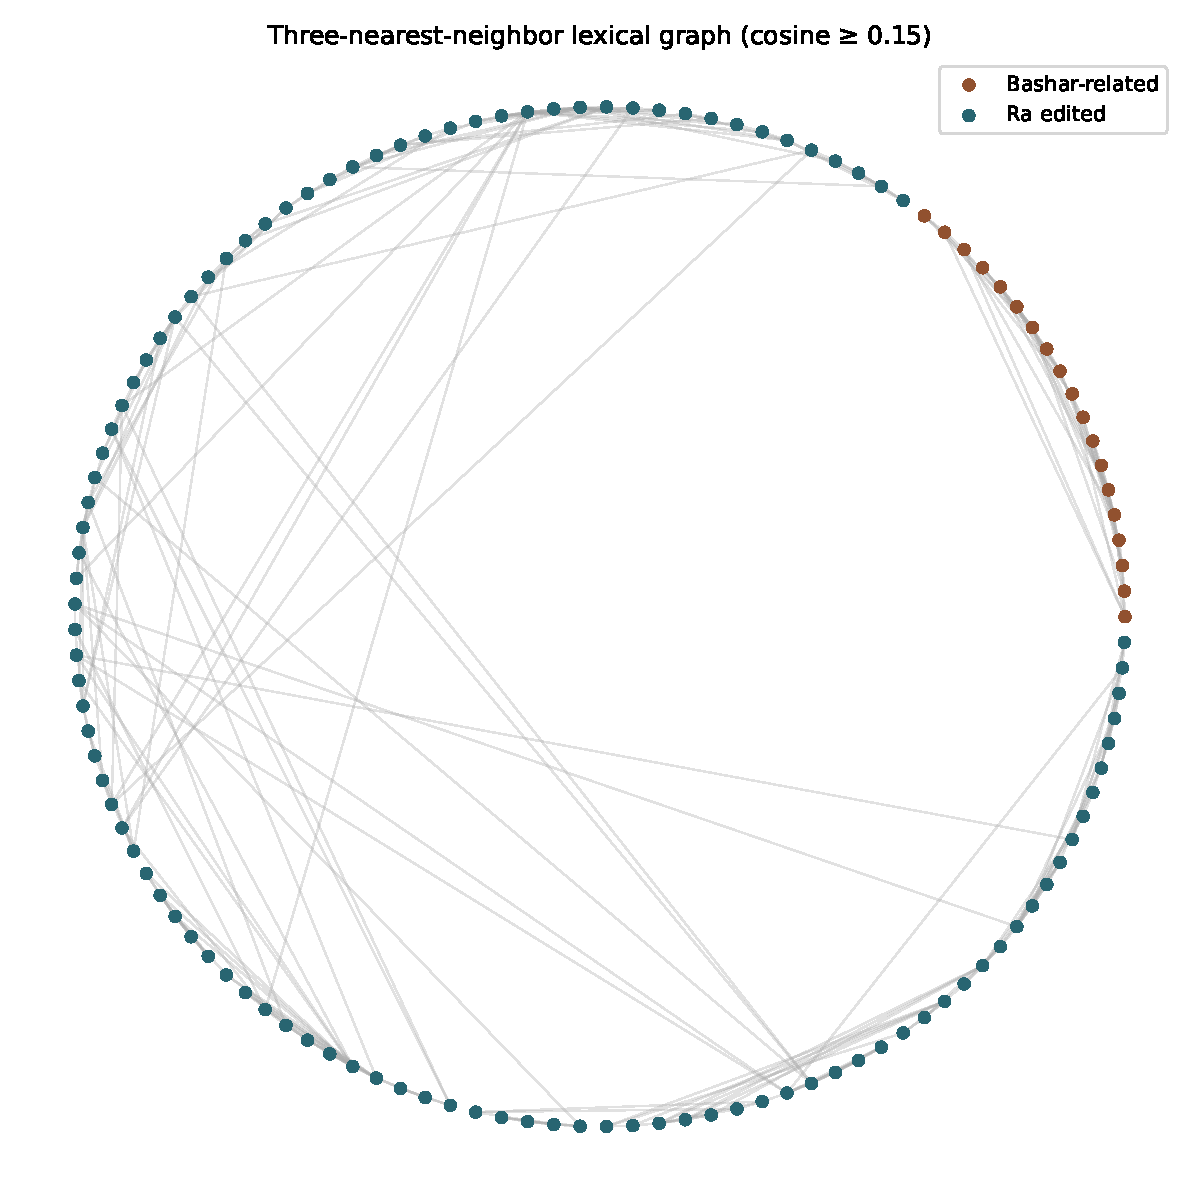
\includegraphics[width=0.95\textwidth,height=\textheight]{figures/lexical-network.pdf}
\caption{Lexical document network. Circular positions are schematic and
the nearest-neighbor/threshold rule determines edges. An absent edge is
not a claim that two documents share no ideas.}
\end{figure}

\FloatBarrier

\subsection{6.5. Neural comparison and documentary
linkage}\label{neural-comparison-and-documentary-linkage}

The corrected frozen MiniLM pass processes 610,730 content wordpieces in
2,611 primary-document chunks, with zero content truncation. Equal-chunk
versus content-token-weighted pooling changes pairwise cosine by a mean
absolute 0.0118, with a maximum change of 0.0806; pair-rank Spearman
correlation is 0.9959. High rank agreement addresses this pooling
choice, not external semantic validity. The neural cosine scale is not
interchangeable with the TF-IDF scale and neither is a probability of
belief agreement.

\begin{figure}
\centering
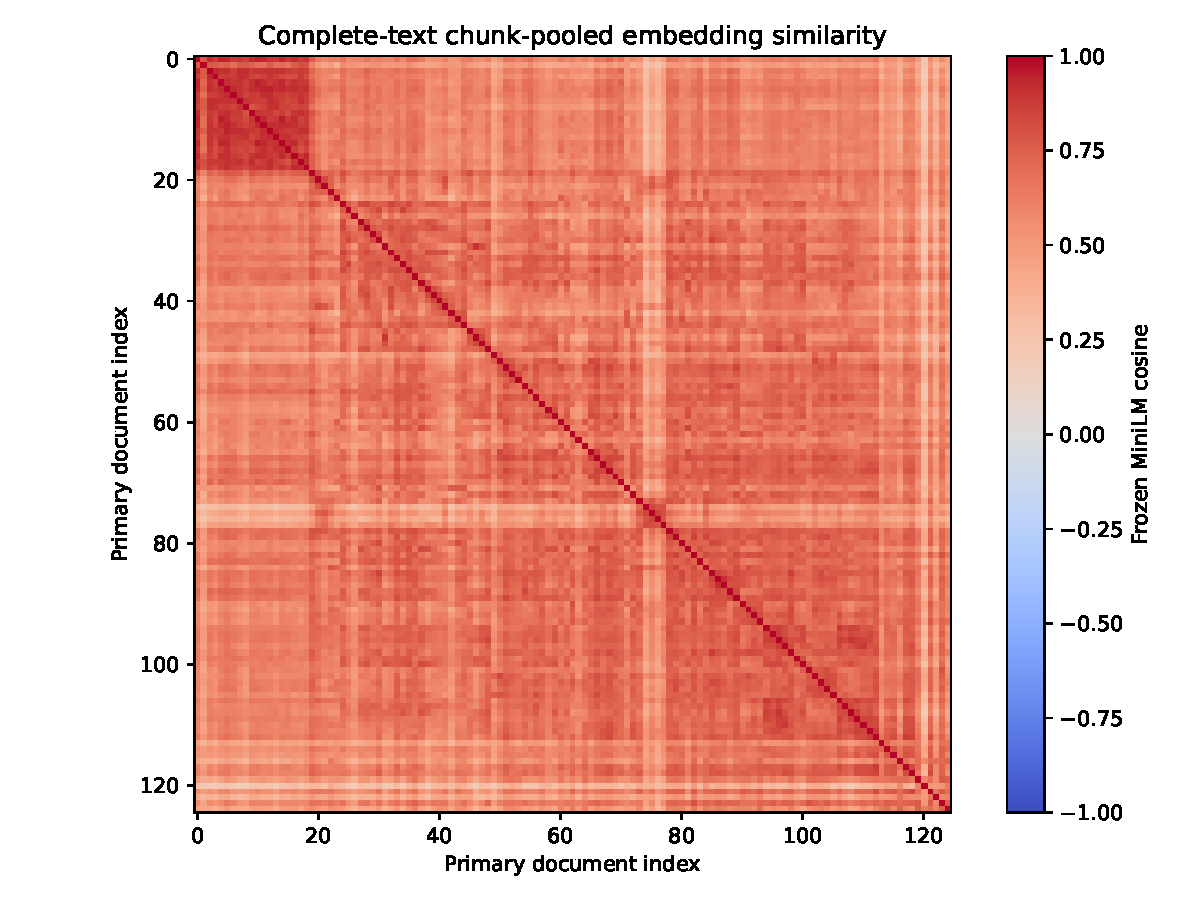
\includegraphics[width=0.85\textwidth,height=\textheight]{figures/semantic-similarity.pdf}
\caption{Frozen neural document cosine matrix. All content wordpieces
are processed under the pinned encoder. Scores remain
representation-dependent and do not authenticate claims or establish
semantic equivalence.}
\end{figure}

The eligible question layer processes 319,281 content wordpieces across
5,397 prompt/response/candidate items, with zero content truncation.
Across 106 Ra sessions, the mean of session-mean matched prompt/response
cosines is 0.3350, versus 0.2068 for one within-session cyclic
reassignment. Every session difference is positive. This supports a
descriptive observation that documentary pairings are more related under
this encoder than that particular reassignment. It does not create a
null distribution, establish statistical significance, certify answer
truth or provide 106 independent experimental replications.

The corrected source-marker filter treats full lexical tokens with
apostrophes intact, preserving contractions such as \emph{don't} rather
than removing an embedded name marker. All source text remains
unchanged. The corrected output is separately hash-pinned; earlier
neural scores are superseded. Contextual reading below was rebound to
actual corrected retrieval identities, including a newly inspected fifth
lead.

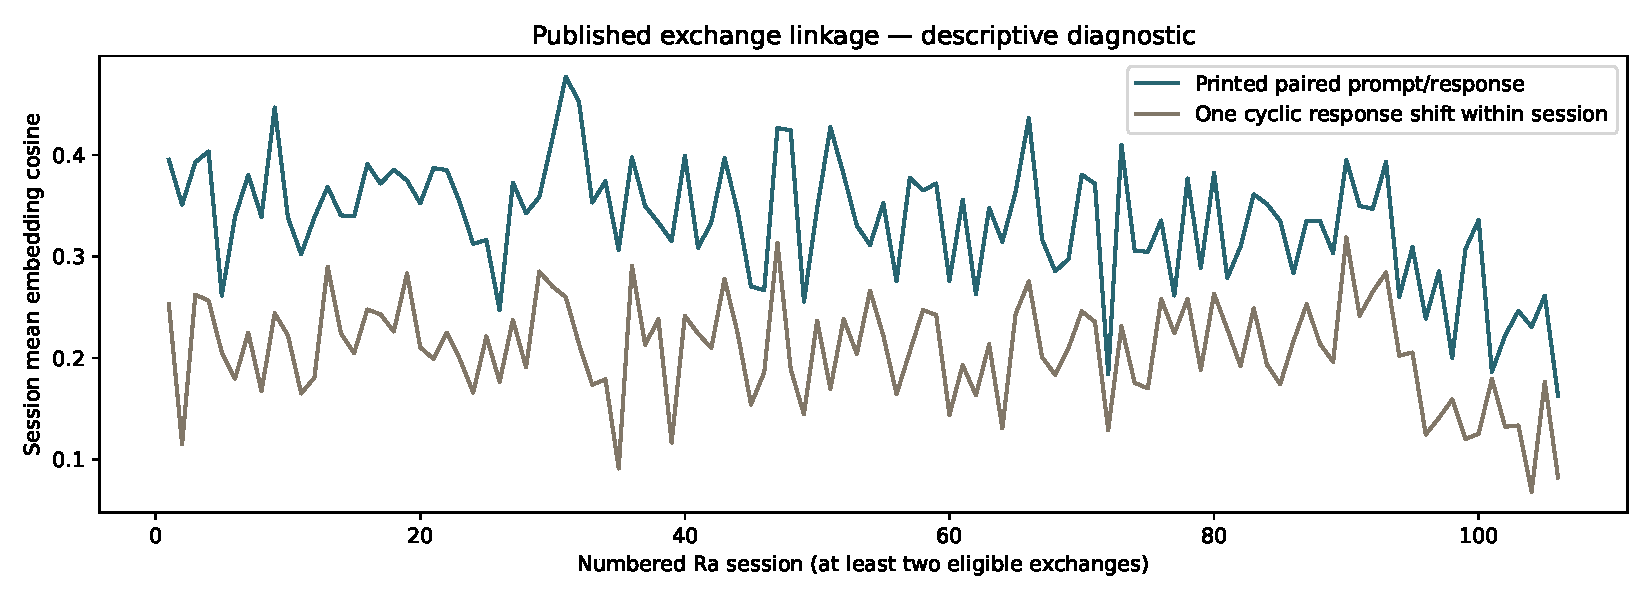
\includegraphics[width=0.95\textwidth,height=\textheight]{figures/question-response-linkage.pdf}

The question database contains 2,523 printed prompt/response exchanges,
including four missing-question placeholders, and 1,303 ASR punctuation
candidates. It also preserves 107 Ra response turns without a present
questioner and 18 bracket-only turns. These are structural units rather
than independently validated substantive questions. For instance, a
printed questioner turn can be an acknowledgment, a request to continue
or a notice that the original question was lost.

\begin{figure}
\centering
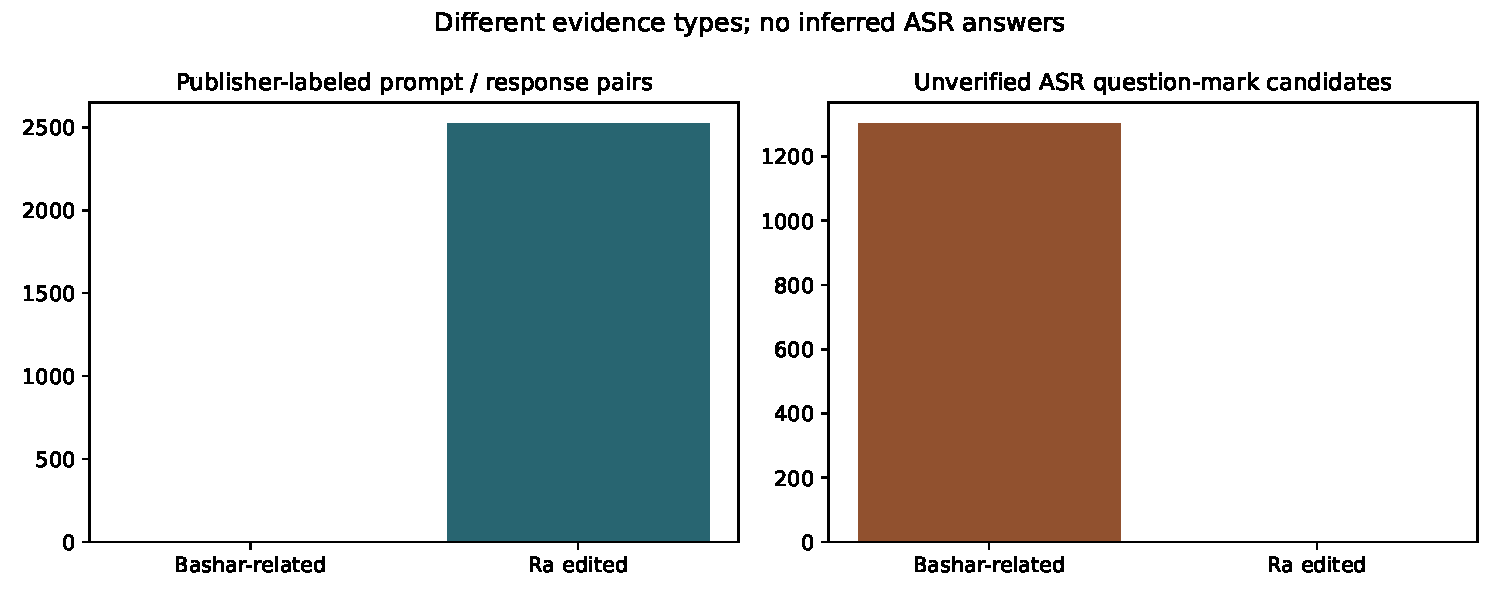
\includegraphics[width=0.9\textwidth,height=\textheight]{figures/qa-structure.pdf}
\caption{Documentary question/response structure and ASR punctuation
candidates. These different extraction mechanisms cannot be interpreted
as comparable rates of verified substantive questions.}
\end{figure}

\FloatBarrier

\subsection{6.6. Contextual retrieval audit illustrates the need for
context}\label{contextual-retrieval-audit-illustrates-the-need-for-context}

The five highest-cosine leads in corrected Run04 were checked against
actual source identities and context. The first four exactly match
previously inspected pairs; the changed fifth received an additional
reading, including the surrounding Ra80.15--80.17 exchanges. The
original pilot receipts and its former Egyptian fifth remain separate
historical evidence. This is not a second independent annotation. The
five selected examples demonstrate failure modes and do not estimate
retrieval precision across the 775 candidates.

\begin{longtable}[]{@{}
  >{\raggedright\arraybackslash}p{(\columnwidth - 4\tabcolsep) * \real{0.1600}}
  >{\raggedright\arraybackslash}p{(\columnwidth - 4\tabcolsep) * \real{0.3800}}
  >{\raggedright\arraybackslash}p{(\columnwidth - 4\tabcolsep) * \real{0.4600}}@{}}
\toprule\noalign{}
\begin{minipage}[b]{\linewidth}\raggedright
Corrected case
\end{minipage} & \begin{minipage}[b]{\linewidth}\raggedright
Source-linked contextual result
\end{minipage} & \begin{minipage}[b]{\linewidth}\raggedright
Why the proposed match is limited
\end{minipage} \\
\midrule\noalign{}
\endhead
\bottomrule\noalign{}
\endlastfoot
Feelings and the body & Ra
\href{https://www.lawofone.info/s/61\#61.7}{61.7};
\href{https://feeds.megaphone.fm/SSM6025167151}{Align \#561 publisher
feed}, ASR 853.34--883.86 s & Broad mind/body family overlap, but
examples of sensations differ from a question about somatic versus
intellectual work; interview response remains incomplete in the
window \\
Spontaneous healing & Ra
\href{https://www.lawofone.info/s/66\#66.12}{66.12};
\href{https://rss.pdrl.fm/a88a08/feeds.megaphone.fm/MASL6091580855/}{Part
Two publisher feed}, ASR 1553.13--1584.89 s & The ASR candidate combines
the end of a prompt with the start of an answer; broad healing language
does not establish matched speaker turns or clinical validity \\
What can be done? & Ra
\href{https://www.lawofone.info/s/104\#104.5}{104.5--104.7};
\href{https://anchor.fm/s/d22ad49c/podcast/rss}{Episode \#248 publisher
feed}, ASR 3088.41--3110.17 s & The Ra context concerns a cat's eyesight
and treatment burden; the interview concerns social abuse \\
Place and negativity & Ra
\href{https://www.lawofone.info/s/106\#106.8}{106.8};
\href{https://rss.pdrl.fm/a88a08/feeds.megaphone.fm/MASL6091580855/}{Part
Two publisher feed}, ASR 656.54--696.42 s & A proposed physical location
is compared with a question about evil and social disillusionment \\
Spirit and roles & Ra
\href{https://www.lawofone.info/s/80\#80.15}{80.15--80.17};
\href{https://feeds.megaphone.fm/acidforsquares}{Episode \#68 publisher
feed}, ASR 4777.41--4807.89 s & A numbered archetypal concept differs
from a comparison between living people's skills and the roles of people
described as being in spirit \\
\end{longtable}

ASR times refer to the retained recording. Publisher-feed links are
source indexes, not guaranteed timestamp players or verified YouTube
editions. Full source titles, IDs and exact intervals are retained in
the machine-readable comparison companion.

The corrected five cosine scores are 0.6784, 0.6767, 0.6739, 0.6677 and
0.6652. The historical Egyptian example, no longer fifth, compares Ra1.5
with an incomplete interview question about the Anunnaki; its original
source reading remains retained rather than erased.

The two generic/referential failures are especially informative. A
sentence asking what can be done has little semantic content without its
antecedent. Similarly, \emph{place} can refer to a location or to a
conceptual role. A nearest-neighbor system can provide a useful lead
while failing precisely at the step required for a comparison of
answers. The database's decision not to infer a Bashar answer from the
next ASR segment is therefore consequential: a single segment can
contain both speakers, and punctuation is insufficient to define
dialogue turns.

\clearpage

\subsection{6.7. Official excerpts add a distinct, bounded
comparison}\label{official-excerpts-add-a-distinct-bounded-comparison}

The admitted 84 English publications comprise 14 platform auto-caption
editions and 70 local-ASR editions. Exact-media grouping leaves 82
units: 14 caption units and 68 ASR units. The following counts describe
model units; all 87 discovery-frame publication dispositions remain
available separately.

\begin{longtable}[]{@{}
  >{\raggedright\arraybackslash}p{(\columnwidth - 6\tabcolsep) * \real{0.3100}}
  >{\raggedleft\arraybackslash}p{(\columnwidth - 6\tabcolsep) * \real{0.1000}}
  >{\raggedleft\arraybackslash}p{(\columnwidth - 6\tabcolsep) * \real{0.1400}}
  >{\raggedright\arraybackslash}p{(\columnwidth - 6\tabcolsep) * \real{0.4500}}@{}}
\toprule\noalign{}
\begin{minipage}[b]{\linewidth}\raggedright
Supplementary stratum
\end{minipage} & \begin{minipage}[b]{\linewidth}\raggedleft
Model units
\end{minipage} & \begin{minipage}[b]{\linewidth}\raggedleft
Whitespace words
\end{minipage} & \begin{minipage}[b]{\linewidth}\raggedright
Analysis role
\end{minipage} \\
\midrule\noalign{}
\endhead
\bottomrule\noalign{}
\endlastfoot
Ordinary official excerpts & 75 & 62,590 & Frozen projection and
separate excerpt-only topic exploration \\
Promotional/product material & 4 & 2,895 & Separate projection stratum;
excluded from excerpt-only topic fit \\
Greetings & 3 & 2,051 & Separate projection stratum; excluded from
excerpt-only topic fit \\
Total admitted model units & 82 & 67,536 & Outside the original
125-document primary fit \\
\end{longtable}

\begin{figure}
\centering
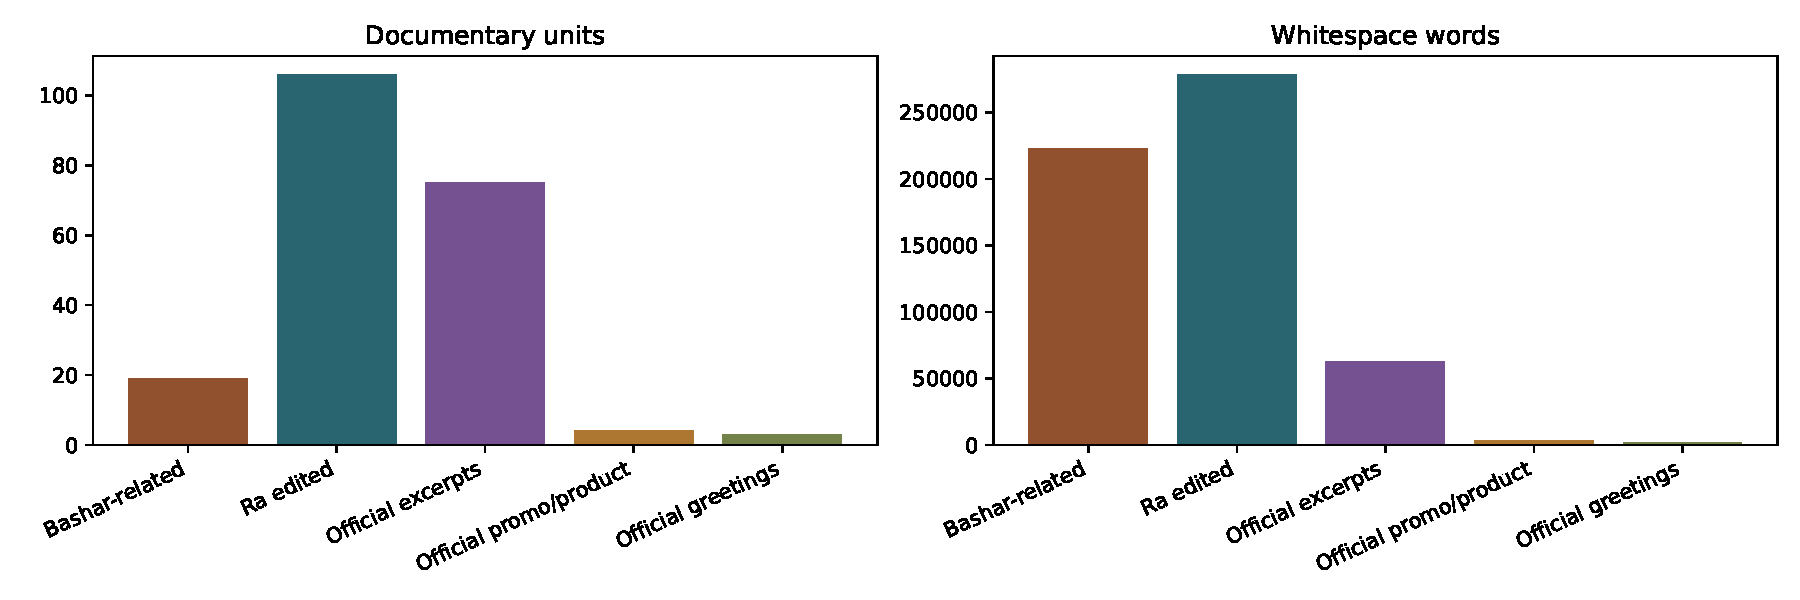
\includegraphics[width=0.95\textwidth,height=\textheight]{figures/official-coverage.pdf}
\caption{The supplementary frame distinguishes original baseline units
from official excerpt, promotional/product and greeting units. English
publication counts are 84 before exact-media grouping; no bar represents
independent creators or complete original sessions.}
\end{figure}

The fixed dictionaries retain their word-form interpretation. Across
ordinary excerpts, equal-unit mean rates per thousand tokens are 9.574
for the agency/free-will list, 5.379 for ethics/polarity, 1.520 for fear
and 10.324 for knowing/uncertainty. The respective pooled-token rates
are 9.521, 5.032, 1.518 and 10.336. Differences between weighting
schemes are observable, but both still count forms rather than annotated
beliefs. In particular, positive/negative vocabulary and conversational
uses of knowing terms require the contextual distinctions demonstrated
in the primary reading audit.

\begin{figure}
\centering
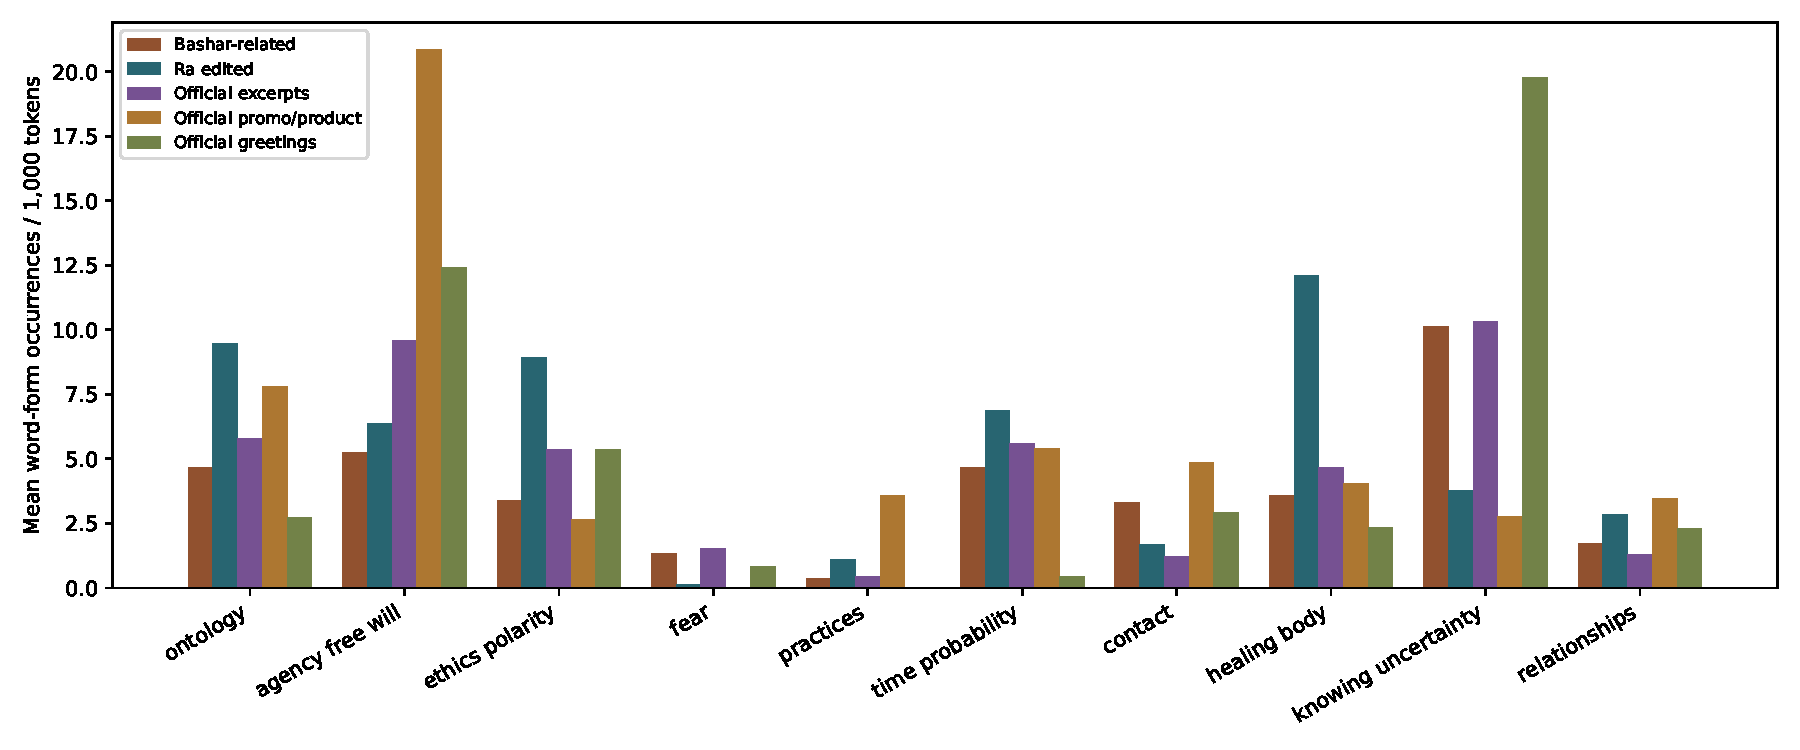
\includegraphics[width=0.95\textwidth,height=\textheight]{figures/official-keywords.pdf}
\caption{Declared keyword families applied to the separate source
strata. Rates are neither endorsement scores nor verified quantities of
discussion about a concept; document weighting and source selection
remain consequential.}
\end{figure}

In frozen baseline TF-IDF space, mean excerpt-to-context cosine is
0.1508 across 1,425 pairs, compared with 0.0531 across 7,950
excerpt-to-Ra pairs. With centered 400-token windows these means are
0.0521 and 0.0220. The same excerpt/context pairing is therefore closer
on average under both stated length conditions, while the score
magnitudes change substantially. These dependent pairs do not provide
independent replications or a causal estimate of doctrinal relatedness.
No projection has a zero retained-feature vector. One short promotional
unit is excluded from the 400-token sensitivity; the 75 ordinary
excerpts, 19 contexts and 106 Ra sessions remain eligible for the two
comparisons below.

\begin{longtable}[]{@{}
  >{\raggedright\arraybackslash}p{(\columnwidth - 4\tabcolsep) * \real{0.5000}}
  >{\raggedleft\arraybackslash}p{(\columnwidth - 4\tabcolsep) * \real{0.2500}}
  >{\raggedleft\arraybackslash}p{(\columnwidth - 4\tabcolsep) * \real{0.2500}}@{}}
\toprule\noalign{}
\begin{minipage}[b]{\linewidth}\raggedright
Representation
\end{minipage} & \begin{minipage}[b]{\linewidth}\raggedleft
Excerpts to mixed contexts
\end{minipage} & \begin{minipage}[b]{\linewidth}\raggedleft
Excerpts to Ra
\end{minipage} \\
\midrule\noalign{}
\endhead
\bottomrule\noalign{}
\endlastfoot
Frozen TF-IDF, full documents & 0.1508 & 0.0531 \\
Frozen TF-IDF, centered 400-token windows & 0.0521 & 0.0220 \\
Frozen MiniLM, full documents & 0.6147 & 0.4478 \\
Frozen MiniLM, centered 400-token source spans & 0.3377 & 0.2791 \\
\end{longtable}

\begin{figure}
\centering
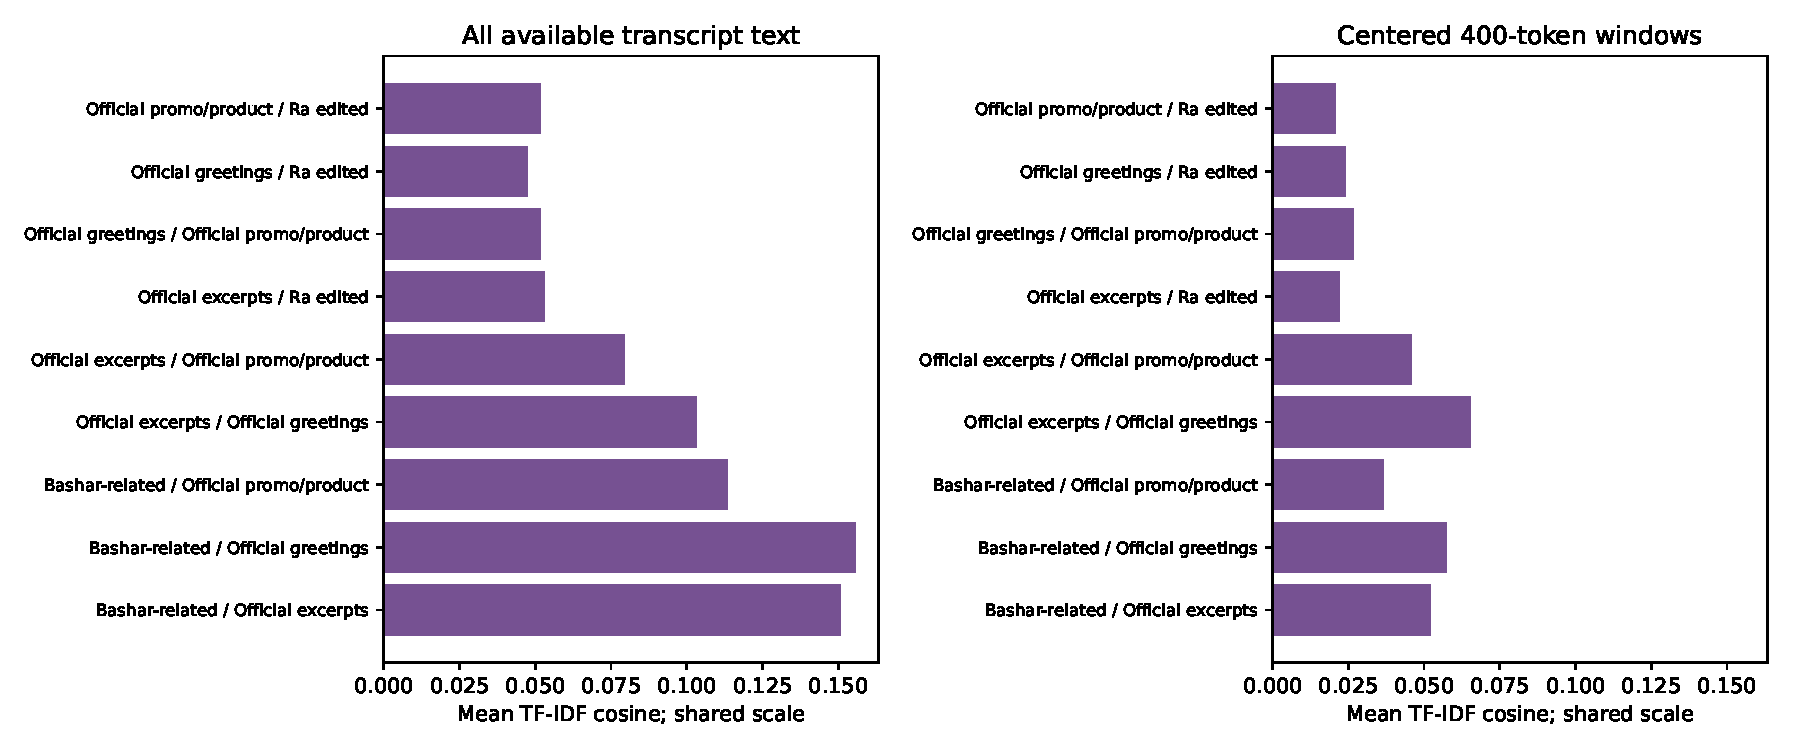
\includegraphics[width=0.95\textwidth,height=\textheight]{figures/official-projection.pdf}
\caption{Official clips projected into the unchanged baseline lexical
space, alongside the centered-window sensitivity. This extends the
source inventory without redefining the original fitted vocabulary or
treating short clips as full sessions.}
\end{figure}

The neural pass covers all 207 combined baseline and official model
units: 690,771 content wordpieces in 2,982 chunks, with no truncation.
Full-document excerpt-to-context and excerpt-to-Ra means are 0.6147 and
0.4478; centered-source-span means are 0.3377 and 0.2791. Neural and
lexical scales must not be read as interchangeable probabilities. Both
offer a source-dependent proximity pattern, while neither tests
equivalent answers, authenticates a voice or establishes the truth of a
claim.

\begin{figure}
\centering
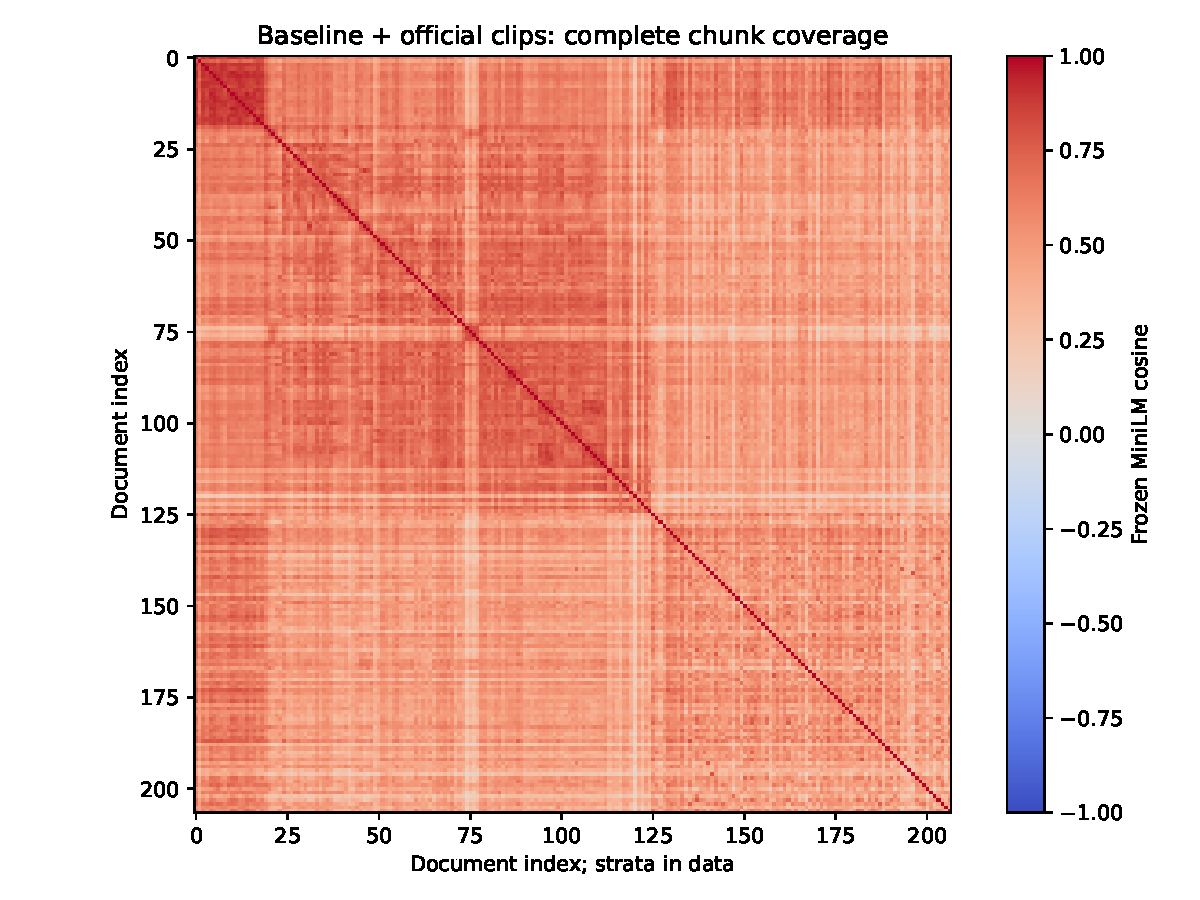
\includegraphics[width=0.95\textwidth,height=\textheight]{figures/official-semantic.pdf}
\caption{Separate neural sensitivity for the official source strata. The
same pinned pretrained model is reused without training; changes between
full documents and bounded source spans show representation and length
dependence.}
\end{figure}

The excerpt-only NMF display separates several top-term families that
were compressed into the primary source-format contrast. Its four mean
normalized component shares are 0.301 for parallel reality/time/contact
terms, 0.362 for positive/negative belief and fear terms, 0.115 for
higher/physical mind and visualization terms, and 0.222 for spirit and
physical-experience terms. These are summaries of top words, not
independently verified thematic labels. The four-component seed-matching
diagnostic is 0.8818, so even the narrow structured-initialization check
is imperfect. All candidate counts from two through eight converge in
this follow-on, but convergence does not select a correct taxonomy.

Internal KMeans partitioning offers especially little basis for
categorical claims. The selected three-cluster fit has sizes 38, 26 and
11, a cosine silhouette of 0.0116 and mean seed adjusted-Rand agreement
of 0.0665. Other candidate counts also have low separation and weak seed
agreement. Thus the source collection supports browsing overlapping word
patterns more convincingly than treating its clusters as stable classes
of teachings.

The two machine-edition comparisons have token edit distances of four
against 606 caption tokens and six against 869 caption tokens,
approximately 0.660\% and 0.690\% respectively. Close agreement between
these two outputs does not establish that either correctly captures the
audio, and two selected pairs cannot estimate accuracy for the
collection. The publication-level database retains 6,736 turns and 479
punctuation-derived question candidates; after exact-media grouping
there are 454 candidates. No answers or speaker turns are authenticated
by this extraction, and no diarization was performed. The only complete
new-excerpt semantic inspection remains the separately documented
870-word time-travel pilot.

\FloatBarrier

\section{7. Source-qualified qualitative
contrasts}\label{source-qualified-qualitative-contrasts}

\FloatBarrier

\subsection{7.1. Unity and responsibility do not imply identical
teachings}\label{unity-and-responsibility-do-not-imply-identical-teachings}

Ra \href{https://www.lawofone.info/s/1\#1.7}{1.7},
\href{https://www.lawofone.info/s/19\#19.1}{19.1} and
\href{https://www.lawofone.info/s/4\#4.20}{4.20} frame unity as
fundamental while describing differentiated experience and development.
Bashar's official \href{https://www.bashar.org/principles}{Principles}
and \href{https://www.bashar.org/fivelaws}{Five Laws} likewise frame
consciousness and physical experience through unity. This supports a
broad passage-level parallel, but the developmental vocabularies are not
interchangeable. The inspected Nine Levels handout groups several
psychological layers within a density; counting nine listed levels does
not establish nine densities or a one-to-one mapping to Ra categories.

Both sources also retain a role for the recipient's choices. Ra
\href{https://www.lawofone.info/s/17\#17.2}{17.2} limits what a teacher
can directly confer, describing inspiration or catalyst rather than
transferable enlightenment. The official Bashar
\href{https://www.bashar.org/message}{Message} presents interaction as
reflection that should preserve human responsibility. Ra
\href{https://www.lawofone.info/s/2\#2.2}{2.2}, however, narrates an
earlier intervention allegedly distorted through elite capture and
accepts responsibility for its effects. That narrative of failure
differs from a statement of current noninterference. Neither establishes
that individuals control all external events.

\FloatBarrier

\subsection{7.2. Practice and emotional work have different operational
forms}\label{practice-and-emotional-work-have-different-operational-forms}

Ra \href{https://www.lawofone.info/s/10\#10.14}{10.14} proposes
attention to love in the moment and recognition of the Creator in other
people, oneself and surrounding creation, supported by contemplation,
meditation or prayer. Bashar's official
\href{https://www.bashar.org/formula}{Formula} links action on
enthusiasm to effort, non-insistence on outcomes, a positive stance and
belief review. \href{https://www.bashar.org/sevensteps}{Seven Steps}
pairs intention and action with allowance. Both offer practical
sequences, but the sequences should not be collapsed into a generic
positive-thinking label.

The same care is needed with difficult feelings. Ra
\href{https://www.lawofone.info/s/18\#18.5}{18.5} recommends examining
and accepting desire rather than suppressing it, while distinguishing
imagination from actions inconsistent with others' free will. The Bashar
Formula recommends investigating fear-based beliefs. The inspected
Spectrum of Fear handout also recognizes a protective role for fear,
which is a direct counterexample to the interpretation that all fear is
inherently harmful. These sources discuss overlapping internal
experiences, not an identical psychological construct or an evaluated
therapeutic intervention.

\FloatBarrier

\subsection{7.3. Time claims change with explanatory
frame}\label{time-claims-change-with-explanatory-frame}

Ra \href{https://www.lawofone.info/s/36\#36.4}{36.4--36.6} permits an
all-at-once frame while rejecting the questioner's simpler
interpretation of simultaneous parts of a self. It describes the higher
self as future-relative from a human space/time standpoint. The Bashar
written references use a one-moment vocabulary and describe past/future
experience as related to the present. It would be misleading to label
these as either a single equivalent theory or a flat contradiction
without retaining their changes of reference frame.

The newly acquired official \href{https://vimeo.com/392834325}{Vimeo
excerpt} provides a more specific Bashar-attributed illustration. Its
ASR at 96.99--125.15 seconds distinguishes a past-like parallel reality
from returning to one's own past. At 164.19--190.82 seconds it describes
a reality perceived as future while claiming simultaneous coexistence.
Later language presents mutual interaction as forming an overlapping
possibility. These passages deepen the comparison of perspectives; they
do not demonstrate time travel, quantify probability or verify an event.

The excerpt also illustrates recognition uncertainty. At 132.83--138.75
seconds the ASR includes wording about being able to duplicate a moment
amid adjacent statements denying duplication. This inconsistency is
retained and flagged, not silently corrected. All 870 output words were
read; no listening-based resolution is claimed. The 422.336-second
public media and its 28.05--376.38-second recognized span are different
coverage measures.

\FloatBarrier

\subsection{7.4. Ethics, contact and health require
counterexamples}\label{ethics-contact-and-health-require-counterexamples}

Ra \href{https://www.lawofone.info/s/18\#18.6}{18.6} describes service
through attention to others' needs and context. Ra
\href{https://www.lawofone.info/s/50\#50.6}{50.6} and
\href{https://www.lawofone.info/s/87\#87.15}{87.15} describe negatively
oriented hierarchy and control within the narrative. The Bashar Message
emphasizes reciprocity, unconditional love and differing belief systems.
These are useful relational parallels, but the word \emph{polarity}
itself is not a reliable moral label: Ra
\href{https://www.lawofone.info/s/45\#45.10}{45.10}, selected by the
ethics dictionary, concerns ears and magnetic terminology.

Contact claims also use different denominators. Ra
\href{https://www.lawofone.info/s/53\#53.15}{53.15} refers to a
preponderance of contacts within its Confederation/Orion framing. A
retained interview's claim about generally positive advanced
civilizations concerns a different population and unresolved speakers.
Treating them as conflicting measured contact rates would manufacture a
comparison neither source supplies. Publisher attribution documents the
claim of communication; it does not authenticate the purported
interlocutor.

For healing, Ra \href{https://www.lawofone.info/s/4\#4.20}{4.20}
presents the healer as a catalyst in an individual process. The Bashar
Message connects changes in self-understanding with physical experience,
but provides no clinical trial or comparable treatment protocol. Ra
\href{https://www.lawofone.info/s/105\#105.4}{105.4} explicitly
describes a particular relapse as physical despite the surrounding
metaphysical account. That passage defeats an indiscriminate reading
that every illness is purely metaphysical. The documents do not justify
attributing illness or harm to a person's beliefs.

\FloatBarrier

\subsection{7.5. Refusal and source framing are part of the
answer}\label{refusal-and-source-framing-are-part-of-the-answer}

Some of the most important observations are absences or corrections in
the response. Ra \href{https://www.lawofone.info/s/77\#77.15}{77.15}
explicitly corrects a questioner's premise;
\href{https://www.lawofone.info/s/68\#68.9}{68.9} declines to answer on
stated free-will grounds;
\href{https://www.lawofone.info/s/96\#96.12}{96.12} supplies no
mechanism for the questioner's proposed hawk-message interpretation. A
system that merges a question and response into a bag of words can make
an unsupported premise look like a supplied explanation.

The interview contexts have a complementary problem. Actual inspected
windows contain commercial or charitable sponsorship, skeptical
retelling, personal anecdote and a statement about teaching the Formula
in one's own voice. Their vocabulary may resemble the teaching while
their speech act and attribution differ. A relationship-themed charity
advertisement is not a doctrinal answer. These counterexamples motivate
retaining source-format and turn uncertainty in retrieval interfaces
instead of displaying one undifferentiated transcript-derived knowledge
base.

\FloatBarrier

\section{8. Discussion}\label{discussion}

\FloatBarrier

\subsection{8.1. What the combined evidence
supports}\label{what-the-combined-evidence-supports}

The quantitative and qualitative layers answer different questions. The
lexical results show that the retained source contexts have different
word distributions and nearest-neighbor structure. The length
sensitivity shows that a substantial part of the observed contrast
depends on the amount and selection of text. The reading layer
identifies passage-level parallels and contrasts that those global
measures cannot establish on their own. In particular, unity and
recipient responsibility recur in the inspected official references,
while practical sequences, time frames and qualifications remain
distinct.

These observations are compatible with multiple explanations. Different
teachings may contribute to the vocabulary patterns, but so may editing,
period, host prompts, advertising, recording length and recognition
errors. The current design does not separate these explanations. With
only two nominal source contexts, adding many turns or overlapping pairs
cannot create an independent population of communicators. A
source-aligned cluster is therefore a finding about this collection, not
a discovery that one doctrine is mathematically distinct from another in
all media.

The retrieval audit offers a concrete design lesson. A useful interface
should show the candidate question together with its preceding referent,
documentary response or uncertain following context, source format and
timestamp. It should support a classification such as \emph{broad
question family}, \emph{different referent}, \emph{response missing} or
\emph{attribution unresolved}. A single number and two shortened
sentences conceal the information most likely to overturn the proposed
match. The accompanying dashboard and private database retain those
distinctions rather than manufacturing a universal Q/A table.

\FloatBarrier

\subsection{8.2. What the new official material
changes}\label{what-the-new-official-material-changes}

The new official excerpts improve access to publisher-attributed speech,
but they do not automatically solve comparability. Short promotional
selections can favor memorable or marketable claims; auto-caption tracks
and local ASR have different recognition processes; several public
publications can derive from one longer session. Their original session
families and selection mechanisms therefore remain important. The
executed supplementary analysis characterizes these excerpts and
projects them into the existing representation while preserving the
primary result. Its length controls retain an average proximity
difference, but its weak internal clusters discourage a definitive topic
taxonomy. The explicit publication/model-unit denominator and
recognition settings make this a more informative source comparison
without making it a matched experiment.

New material can also modify an interpretation without invalidating the
audit trail. The official time-travel excerpt adds a distinction between
a past-like parallel reality and one's own past. That distinction
qualifies a simplified reading of the short written principles. It does
not retrospectively change what the original model saw, and it does not
justify silently replacing an inconvenient result. Versioned inputs,
separate attestations and living-paper sections make such updates
visible.

\FloatBarrier

\section{9. Limitations}\label{limitations}

\textbf{Sampling and source dependence.} The Ra frame is complete for
one selected published edition; the retained Bashar-related recordings
are a convenience collection of publisher contexts. Neither defines all
available videos, tapes, speakers or historical sessions. Publication
dates are not uniformly event dates, and original-session identity is
unresolved for some material. Exact-hash and five-token screens do not
detect all latent duplication.

\textbf{Confounded comparison.} Corpus label coincides with period,
editing, genre, dialogue structure and recognition process. The lexical
controls address selected observable features but cannot identify a
causal doctrinal effect. Joint vocabulary and IDF also reflect the
unequal 106-versus-19 document counts. Pair counts are not independent
sample sizes, and the two source contexts cannot support general
population claims about channeling.

\textbf{Recognition and editorial uncertainty.} ASR has not received a
stratified listening audit, speaker diarization or systematic
advertisement segmentation. A transcript can contain incorrect negation,
fabricated phrases or mixed speaker turns. Ra editorial roles and
reconstruction improve documentary structure without authenticating a
voice or restoring missing original audio. The handout exclusions show
that a text extraction is not equivalent to complete visual
understanding.

\textbf{Model and selection limits.} Exact dictionary forms are not
validated semantic labels. TF-IDF ignores much compositional meaning;
embeddings and chunk pooling can overlook negation, temporal scope or
antecedents. NMF display count is chosen for readability, its seed
checks use closely related initializations, and one candidate does not
converge. KMeans silhouette is low, the SVD view retains little
variance, and network edges depend on a declared filtering rule. The
corrected neural masking implementation is versioned separately from the
historical retrieval audit. The official excerpt-only clustering is also
weak and seed-sensitive; four displayed NMF word families are
exploratory components, not an externally validated taxonomy.

\textbf{Limited interpretation coverage.} Only small portions of the
original corpora received semantic reading, with deliberate enrichment
and follow-up selection. This increases the chance of finding a useful
example but cannot estimate population prevalence, typicality or
retrieval precision. All readings in this increment are model-assisted;
no human reliability study or complete expert review has occurred.
Apparent differences may also depend on passages not yet inspected.

\textbf{External validity and rights.} This study measures text and
source structure. It does not establish historical accuracy, therapeutic
effectiveness, paranormal phenomena or the identity of a purported
interlocutor. Source availability does not establish permission to
redistribute full texts or train a model. No clinical, physical or
predictive experiment is reported.

\FloatBarrier

\section{10. Planned validation and living-paper
agenda}\label{planned-validation-and-living-paper-agenda}

The following distinguishes completed first steps from proposed
validation studies. Any future confirmatory protocol should be fixed
before interpreting outcomes.

\begin{longtable}[]{@{}
  >{\raggedright\arraybackslash}p{(\columnwidth - 4\tabcolsep) * \real{0.2400}}
  >{\raggedright\arraybackslash}p{(\columnwidth - 4\tabcolsep) * \real{0.4800}}
  >{\raggedright\arraybackslash}p{(\columnwidth - 4\tabcolsep) * \real{0.2800}}@{}}
\toprule\noalign{}
\begin{minipage}[b]{\linewidth}\raggedright
Planned work
\end{minipage} & \begin{minipage}[b]{\linewidth}\raggedright
Concrete design and comparison
\end{minipage} & \begin{minipage}[b]{\linewidth}\raggedright
Status
\end{minipage} \\
\midrule\noalign{}
\endhead
\bottomrule\noalign{}
\endlastfoot
Human source and ASR audit & Sample by publisher, format, duration and
recognition source; compare bounded audio spans with transcript;
annotate speaker changes, advertisements, negation, names and numbers &
\textbf{TBD}; no error rate currently available \\
Human question-family evaluation & Independently label a stratified
sample of retrieval leads and non-leads; distinguish common family,
equivalent proposition, different referent and insufficient context &
\textbf{TBD}; no current precision or agreement estimate \\
Stronger format matching & Extend the completed official-publication
projections and 400-token controls to independently checked speaker
roles and matched Ra response passages & Projection/length study
complete; role-matched validation \textbf{TBD} \\
Session-family resolution & Identify excerpt/repost/edition families
through provenance and bounded content review before any train/test
split & \textbf{TBD}; exact-media families alone are insufficient \\
Broader topic sensitivity & Resample at source/session-family level,
vary vocabulary and initialization families, and compare component
interpretation on held-out passages & \textbf{TBD}; current seed
matching is narrower \\
Role-aware retrieval & Evaluate complete question/context blocks and
explicitly identified answers against segment-level retrieval; retain
refusals and unknown speakers & \textbf{TBD}; current database supports
this distinction \\
Claim-level comparison & Record each proposition's scope, modality,
negation, reference frame and counterexamples; test whether claimed
parallels survive contextual review & Initial examples available;
systematic evaluation \textbf{TBD} \\
Grounded question answering & Retrieve source passages with exact
citations and uncertainty/attribution labels; evaluate answer
faithfulness and abstention on unresolved cases & \textbf{TBD}; no
fine-tuning or new model weights claimed \\
\end{longtable}

A future forecasting study would require dated claims, a prespecified
outcome definition, a complete claim-selection rule, comparison
baselines and blinded outcome coding. A future health study would
require a separate clinically appropriate design and evidence. Neither
can be inferred from lexical similarity, a topic component or an
evocative anecdote. These possibilities are mentioned to define the
boundary of the present work, not to imply that its data already support
such conclusions.

\FloatBarrier

\section{11. Reproducibility and
availability}\label{reproducibility-and-availability}

The repository retains acquisition adapters, analysis code, tests, the
living manuscript, a bibliography and figures. Each accepted analysis
run binds its script, source manifests and output artifacts. The primary
analysis unit is the complete retained document; tokens, chunks, turns
and overlapping pairs are not promoted to independent observations. The
compiled paper and dashboard publish only the approved metadata/results
layer. The full private SQLite Q/A database, source media, substantial
transcript excerpts and model caches remain outside the public release.

The environment versions recorded for the analysis include NumPy 2.3.5,
SciPy 1.17.0, scikit-learn 1.8.0, Matplotlib 3.10.8 and ONNX Runtime
1.23.2. The frozen MiniLM weights are reused without training. Automated
invariant tests and model-agent review address code and provenance
consistency; they are not human peer review or evidence of ASR accuracy.
Paper generation uses Pandoc and pdfLaTeX, with source and build scripts
included. \texttt{snapshot.json} records the exact baseline and separate
final official-study analysis/figure hashes used by the paper. The older
15-publication pilot stays pinned as historical evidence rather than
being relabeled as final-frame coverage.

For the original source-reading evidence, the initial selection and its
completed-reading attestation are separate artifacts. A later follow-up
records new inspected intervals without overwriting the initial
selection. The public comparison JSON links paraphrases to
session/question IDs or ASR seconds. The methodological reference note
records actual page/abstract access depth. These contracts allow later
readers to distinguish acquisition, computation, interpretation and
validation as the project grows.

\FloatBarrier

\section{12. Conclusion}\label{conclusion}

The retained Ra and Bashar-related materials can be compared
reproducibly, but their production contexts must remain part of the
analysis. Their lexical distributions and fitted components differ, and
several source-linked passages share unity-oriented or agency-related
themes. Those observations do not establish equivalent teachings or a
common origin. The larger official-publication follow-on retains
source-dependent proximity under length controls but produces weak
internal clusters. Document-length sensitivity, editorial structure,
mixed speakers and contextual retrieval failures materially limit
stronger conclusions. A useful research resource preserves those limits
while making the underlying examples, exclusions and future validation
tasks easier to inspect.

\clearpage

\section*{References}\label{references}
\addcontentsline{toc}{section}{References}

\phantomsection\label{refs}
\begin{CSLReferences}{1}{0}
\bibitem[\citeproctext]{ref-bender2018}
Bender, Emily M., and Batya Friedman. 2018. {``Data Statements for
Natural Language Processing: Toward Mitigating System Bias and Enabling
Better Science.''} \emph{Transactions of the Association for
Computational Linguistics} 6: 587--604.
\url{https://doi.org/10.1162/tacl_a_00041}.

\bibitem[\citeproctext]{ref-doogan2021}
Doogan, Caitlin, and Wray Buntine. 2021. {``Topic Model or Topic
Twaddle? Re-Evaluating Semantic Interpretability Measures.''} In
\emph{Proceedings of the 2021 Conference of the North American Chapter
of the Association for Computational Linguistics: Human Language
Technologies}, 3824--48.
\url{https://doi.org/10.18653/v1/2021.naacl-main.300}.

\bibitem[\citeproctext]{ref-kapoor2023}
Kapoor, Sayash, and Arvind Narayanan. 2023. {``Leakage and the
Reproducibility Crisis in Machine-Learning-Based Science.''}
\emph{Patterns} 4 (9): 100804.
\url{https://doi.org/10.1016/j.patter.2023.100804}.

\bibitem[\citeproctext]{ref-koenecke2024}
Koenecke, Allison, Anna Seo Gyeong Choi, Katelyn X. Mei, Hilke
Schellmann, and Mona Sloane. 2024. {``Careless Whisper: Speech-to-Text
Hallucination Harms.''} In \emph{The 2024 ACM Conference on Fairness,
Accountability, and Transparency}, 1672--81.
\url{https://doi.org/10.1145/3630106.3658996}.

\bibitem[\citeproctext]{ref-schroeder2025}
Schroeder, Kayla, and Zach Wood-Doughty. 2025. {``Reliability of Topic
Modeling.''} In \emph{Proceedings of the 2025 Conference of the Nations
of the Americas Chapter of the Association for Computational
Linguistics: Human Language Technologies}, 2649--62.
\url{https://doi.org/10.18653/v1/2025.naacl-long.134}.

\end{CSLReferences}

\end{document}
